\documentclass[10pt]{beamer}

\usetheme{metropolis}

\usepackage[export]{adjustbox}
\usepackage{array}
\usepackage{etoolbox}
\usepackage{graphicx}
\usepackage{hyperref}
\usepackage{listings}
\usepackage{pgfplots}
\usepackage{pgfplotstable}
\usepackage{tikz}
\usepackage{xcolor}

\usepgfplotslibrary{fillbetween}
\usepgfplotslibrary{groupplots}
\usepgfplotslibrary{statistics}

\usetikzlibrary{arrows.meta}
\usetikzlibrary{calc}
\usetikzlibrary{fillbetween}
\usetikzlibrary{patterns}
\usetikzlibrary{positioning}

\hypersetup{
    colorlinks=true,
    linkcolor=white,
    urlcolor=blue!80
}

\definecolor{uiored}{HTML}{DD0000}
\definecolor{uiolightred}{HTML}{FB6666}
\definecolor{uioredtone}{HTML}{FEE0E0}
\definecolor{uioblue}{HTML}{3E31D6}
\definecolor{uiolightblue}{HTML}{86A4F7}
\definecolor{uioblueone}{HTML}{E6ECFF}
\definecolor{uiogreen}{HTML}{2EC483}
\definecolor{uiolightgreen}{HTML}{6CE1AB}
\definecolor{uiogreentone}{HTML}{CEFFDF}
\definecolor{uioorange}{HTML}{FEA11B}
\definecolor{uiolightorange}{HTML}{FDCB87}
\definecolor{uioorangetone}{HTML}{FFE8D4}
\definecolor{uioyellow}{HTML}{FFFEA7}
\definecolor{uiogray}{HTML}{B2B3B7}

\colorlet{mainbackground}{uiored}

\setbeamercolor{frametitle}{bg=mainbackground, fg=white}
\setbeamercolor{title separator}{fg=mainbackground}
\setbeamercolor{progress bar in section page}{fg=white, bg=uiogray}

\def\logowidth{4cm}

\makeatletter
\setbeamertemplate{section page}
{
  \begingroup

    \vspace{4.3cm}
    {\usebeamercolor[fg]{section title}\usebeamerfont{section title}\insertsectionhead}\\[-1ex]
    {\centering\color{white}\rule{\linewidth}{1pt}\par} % the horizontal line

    \vspace*{3.1cm}
    \begin{center}
        
\includegraphics[width=\logowidth,valign=c]{data/uio_logo_full_white.png} % Adjust width and path to your logo as needed
    \end{center}

  \endgroup
}
\makeatother

\AtBeginSection{
  {
    \setbeamercolor{background canvas}{bg=uiored}
    \setbeamercolor{section title}{fg=white}
    \frame[plain,c,noframenumbering]{\sectionpage}
    \setbeamercolor{background canvas}{bg=black!2}
  }
}



\setbeamertemplate{footline}{
    \ifnum\insertframenumber=1
        % Title page, no footer
    \else
        \begin{tikzpicture}[remember picture,overlay]
            \fill[mainbackground] (current page.south west) rectangle ([yshift=0.45cm]current page.south east); % Draw filled rectangle

            % Logo
            \node[anchor=west, yshift=0.225cm] at (current page.south west) {
\includegraphics[height=1.2cm]{data/uio_logo_white.png}};

            % Title and subtitle
            \node[align=center, yshift=0.225cm] at (current page.south) {\textcolor{white}{\textbf{\inserttitle}}\\[0.05cm]\textcolor{white}{\insertsubtitle}};

            % Page number
            \node[anchor=east, yshift=0.225cm, xshift=-0.2cm, align=right] at (current page.south east) {\textcolor{white}{\insertframenumber/\inserttotalframenumber}};
        \end{tikzpicture}
    \fi
}

\subtitle{The role of neuroimaging beyond T1-weighted MRI in the diagnosis and prediction of neuropsychiatric disorders}
\author{Esten H. Leonardsen}
\date{26.10.23}

\definecolor{color1}{HTML}{f94144}
\definecolor{color2}{HTML}{f3722c}
\definecolor{color3}{HTML}{f8961e}
\definecolor{color4}{HTML}{f9c74f}
\definecolor{color5}{HTML}{90be6d}
\definecolor{color6}{HTML}{43aa8b}
\definecolor{color7}{HTML}{577590}

\titlegraphic{
	\centering
	\vspace{7.7cm}
	
\includegraphics[width=\logowidth]{data/uio_logo_full.png}
}

\begin{document}
	\begin{frame}
	 	\titlepage
	\end{frame}

    % \begin{frame}{Overview}
    %     \begin{enumerate}
    %         \item Background: Defining the scope of the lecture.
    %         \item State-of-the-art: How is neuroimaging beyond T1-weighted MRI currently being used with respect to neuropsychiatric disorders.
    %         \item The future: Challenges and opportunities in using neuroimaging for predicting neuropsychiatric disorders moving forward.
    %     \end{enumerate}
    % \end{frame}

    % \newsavebox{\modalities}
    % \sbox{\modalities}{%
    %     \begin{tikzpicture}
    %         \begin{axis}[
    %             ybar,
    %             height=5cm,
    %             width=6cm,
    %             bar width=0.8,
    %             xmin=0.35,
    %             xmax=5.65,
    %             ymin=0,
    %             xtick={1, 2, 3, 4, 5},
    %             xticklabels={sMRI,fMRI,dMRI,Molecular,Elecrophysiological},
    %             x tick label style={
    %                 rotate=45,anchor=east,
    %                 font=\footnotesize
    %             },
    %             tick label style={
    %                 font=\footnotesize
    %             },
    %             ylabel={\footnotesize{Publications}},
    %             ymax=399,
    %             axis y line*=left,
    %             axis x line*=bottom,
    %             xtick align=outside
    %         ]
    %             \addplot[fill=gray!80] coordinates {
    %                 (1, 367)
    %                 (2, 186)
    %                 (3, 39)
    %                 (4, 43)
    %                 (5, 15)
    %             };
    %         \end{axis}
    %     \end{tikzpicture}
    % }

    % \newsavebox{\colouredmodalities}
    % \sbox{\colouredmodalities}{%
    %     \begin{tikzpicture}
    %         \begin{axis}[
    %             ybar stacked,
    %             height=5cm,
    %             width=6cm,
    %             bar width=0.8,
    %             xmin=0.35,
    %             xmax=5.65,
    %             ymin=0,
    %             xtick={1, 2, 3, 4, 5},
    %             xticklabels={sMRI,fMRI,dMRI,Molecular,Elecrophysiological},
    %             x tick label style={
    %                 rotate=45,anchor=east,
    %                 font=\footnotesize
    %             },
    %             tick label style={
    %                 font=\footnotesize
    %             },
    %             ylabel={\footnotesize{Publications}},
    %             ymax=399,
    %             axis y line*=left,
    %             axis x line*=bottom,
    %             xtick align=outside
    %         ]
    %             \addplot[fill=color1] coordinates {
    %                 (1, 124)
    %                 (2, 12)
    %                 (3, 7)
    %                 (4, 23)
    %                 (5, 0)
    %             };
    %             \addplot[fill=color2] coordinates {
    %                 (1, 45)
    %                 (2, 4)
    %                 (3, 1)
    %                 (4, 0)
    %                 (5, 2)
    %             };
    %             \addplot[fill=color3] coordinates {
    %                 (1, 10)
    %                 (2, 1)
    %                 (3, 0)
    %                 (4, 12)
    %                 (5, 0)
    %             };
    %             \addplot[fill=color4] coordinates {
    %                 (1, 68)
    %                 (2, 96)
    %                 (3, 10)
    %                 (4, 0)
    %                 (5, 4)
    %             };
    %             \addplot[fill=color5] coordinates {
    %                 (1, 15)
    %                 (2, 34)
    %                 (3, 9)
    %                 (4, 0)
    %                 (5, 9)
    %             };
    %             \addplot[fill=color6] coordinates {
    %                 (1, 9)
    %                 (2, 5)
    %                 (3, 2)
    %                 (4, 0)
    %                 (5, 0)
    %             };
    %             \addplot[fill=color7] coordinates {
    %                 (1, 96)
    %                 (2, 34)
    %                 (3, 10)
    %                 (4, 8)
    %                 (5, 0)
    %             };
    %         \end{axis}
    %     \end{tikzpicture}
    % }

    % \newsavebox{\casehippo}
    % \sbox{\casehippo}{%
    %     \begin{tikzpicture}
    %         \begin{axis}[
    %             width=4cm,
    %             height=4cm,
    %             ymajorticks=false,
    %             xmin=2491,
    %             xmax=11269,
    %             xtick pos=bottom,
    %             axis x line*=bottom,
    %             hide y axis,
    %             ymin=0,
    %             xtick={4000, 7000, 10000},
    %             scaled x ticks=false,
    %             ticklabel style = {font=\scriptsize},
    %             xlabel={\scriptsize{$mm^3$}},
    %             x label style={at={(axis description cs:0.5,-0.15)},anchor=north},
    %             ymax=0.0005,
    %             clip=false
    %         ]
    %             \addplot[name path=zero] coordinates {
    %                 (2491, 0) (11269, 0)
    %             };
    %             \addplot[
    %                 color1,
    %                 thick,
    %                 name path=case
    %             ] table [
    %                 x=volume,
    %                 y=AD,
    %                 col sep=comma
    %             ] {data/hippocampus_traces.csv};
    %             \tikzfillbetween[of=zero and case]{color1, opacity=0.5};
    %             \node[draw=color1,fill=color1!50, inner sep=2pt,label=right:{\scriptsize{DEM}}] at (axis cs: 10000, 0.0004) {};
    %         \end{axis}
    %     \end{tikzpicture}
    % }

    % \newsavebox{\hippo}
    % \sbox{\hippo}{%
    %     \begin{tikzpicture}
    %         \begin{axis}[
    %             width=4cm,
    %             height=4cm,
    %             ymajorticks=false,
    %             xmin=2491,
    %             xmax=11269,
    %             xtick pos=bottom,
    %             axis x line*=bottom,
    %             hide y axis,
    %             ymin=0,
    %             xtick={4000, 7000, 10000},
    %             scaled x ticks=false,
    %             ticklabel style = {font=\scriptsize},
    %             xlabel={\scriptsize{$mm^3$}},
    %             x label style={at={(axis description cs:0.5,-0.15)},anchor=north},
    %             ymax=0.0005,
    %             clip=false
    %         ]
    %             \addplot[name path=zero] coordinates {
    %                 (2491, 0) (11269, 0)
    %             };
    %             \addplot[
    %                 color1,
    %                 thick,
    %                 name path=case
    %             ] table [
    %                 x=volume,
    %                 y=AD,
    %                 col sep=comma
    %             ] {data/hippocampus_traces.csv};
    %             \addplot[
    %                 color6,
    %                 thick,
    %                 name path=control
    %             ] table [
    %                 x=volume,
    %                 y=CN,
    %                 col sep=comma
    %             ] {data/hippocampus_traces.csv};
    %             \tikzfillbetween[of=zero and case]{color1, opacity=0.5};
    %             \tikzfillbetween[of=zero and control]{color6, opacity=0.5};
    %             \node[draw=color1,fill=color1!50, inner sep=2pt,label=right:{\scriptsize{DEM}}] at (axis cs: 10000, 0.0004) {};
    %             \node[draw=color6,fill=color6!50, inner sep=2pt,label=right:{\scriptsize{HC}}] at (axis cs: 10000, 0.00035) {};
    %         \end{axis}
    %     \end{tikzpicture}
    % }

    % \newsavebox{\hippoauc}
    % \sbox{\hippoauc}{%
    %     \begin{tikzpicture}
    %         \begin{axis}[
    %             width=4cm,
    %             height=4cm,
    %             xmin=0,
    %             xmax=1,
    %             ymin=0,
    %             ymax=1,
    %             ticklabel style = {font=\scriptsize},
    %             xtick={0, 0.25, 0.5, 0.75, 1},
    %             ytick={0, 0.25, 0.5, 0.75, 1},
    %             xtick pos=bottom,
    %             ytick pos=left,
    %             xlabel=\scriptsize{fpr},
    %             ylabel=\scriptsize{tpr},
    %             x label style={at={(axis description cs:0.5,-0.15)},anchor=north},
    %             y label style={at={(axis description cs:-0.25,.5)},anchor=south},
    %         ]
    %         \addplot[draw=none, name path=zero] coordinates {
    %             (0, 0)
    %             (1, 0)
    %         };
    %         \addplot[
    %             color7,
    %             very thick,
    %             name path=roc
    %         ] table [
    %             x=fpr,
    %             y=tpr,
    %             col sep=comma
    %         ] {data/hippocampus_roc.csv};
    %         \tikzfillbetween[of=zero and roc]{color7, opacity=0.75};
    %         \node[anchor=south east] at (axis cs: 0.97, 0.02) {\textcolor{white}{\scriptsize{accuracy=0.81}}};
    %         \end{axis}
    %     \end{tikzpicture}
    % }

    % \begin{frame}[t]{Background}
    %     \centering
    %     \begin{tikzpicture}
    %         \colorlet{hiddencolour}{black!20}

    %         \def\labelsize{\scriptsize}

    %         \node[] at (0, 0) {};
    %         \node[draw=black] at (-5, 0) {};
    %         \node[draw=black] at (5, -7) {};
    %         \onslide<1>{
    %             \node[align=center] at (0, -0.5) {
    %                 The role of neuroimaging beyond T1-weighted MRI in the\\diagnosis and prediction of neuropsychiatric disorders
    %             };
    %         }
    %         \only<2-6>{
    %             \node[align=center] at (0, -0.5) {
    %                 \textcolor{hiddencolour}{The role of }neuroimaging \textcolor{hiddencolour}{beyond T1-weighted MRI in the}\\\textcolor{hiddencolour}{diagnosis and prediction of neuropsychiatric disorders}
    %             };
    %             \onslide<3->{
    %                 \node[inner sep=0pt, label=below:{\labelsize{Bert from FreeSurfer 7.3}}] at (-3, -4) {
    %                     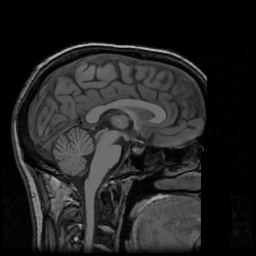
\includegraphics[width=3cm]{data/bert_sagittal.png}
    %                 };
    %             }
    %             \onslide<4->{
    %                 \node[label=below:{\labelsize{Sample from the MNE library}}] at (1.5, -2.5) {
    %                     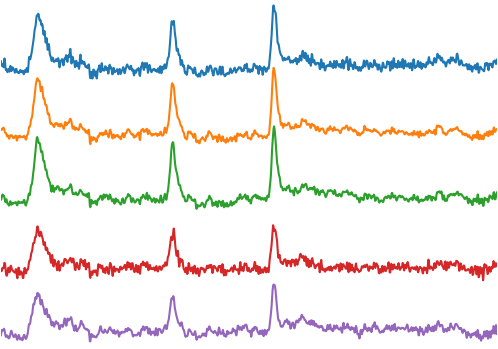
\includegraphics[width=3.75cm]{data/eeg.png}
    %                 };
    %             }
    %             \onslide<5->{
    %                 %https://www.ncbi.nlm.nih.gov/pmc/articles/PMC4980915/
    %                 \node[label=below:{\labelsize{Sample from Tremlay et al., 2016}}] at (0.7, -5.1) {
    %                     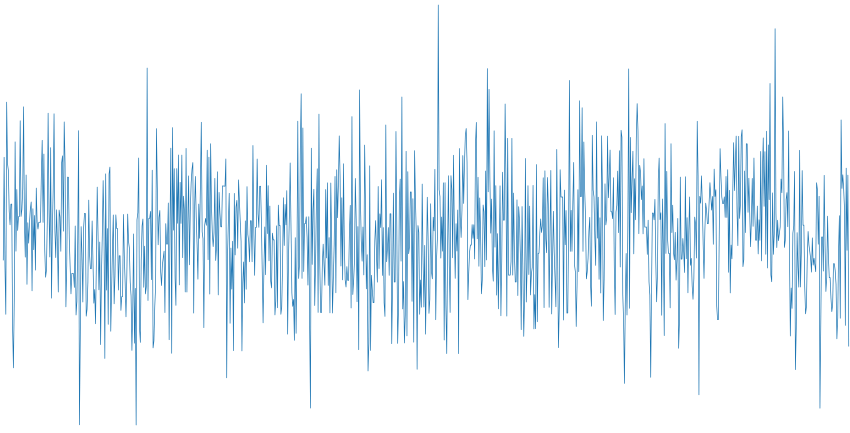
\includegraphics[width=3cm]{data/patch_clamp.png}
    %                 };
    %                 \node[font=\tiny, align=center, anchor=south] at (0, -7.75) {
    %                     Tremblay, R., Lee, S., \& Rudy, B. (2016). GABAergic interneurons in the neocortex: from cellular properties to circuits. Neuron,\\91(2), 260-292
    %                 };
    %             }
    %             \onslide<6->{
    %                 \node[label=below:{\labelsize{Meta Quest Pro}}] at (3.75, -6.1) {
    %                     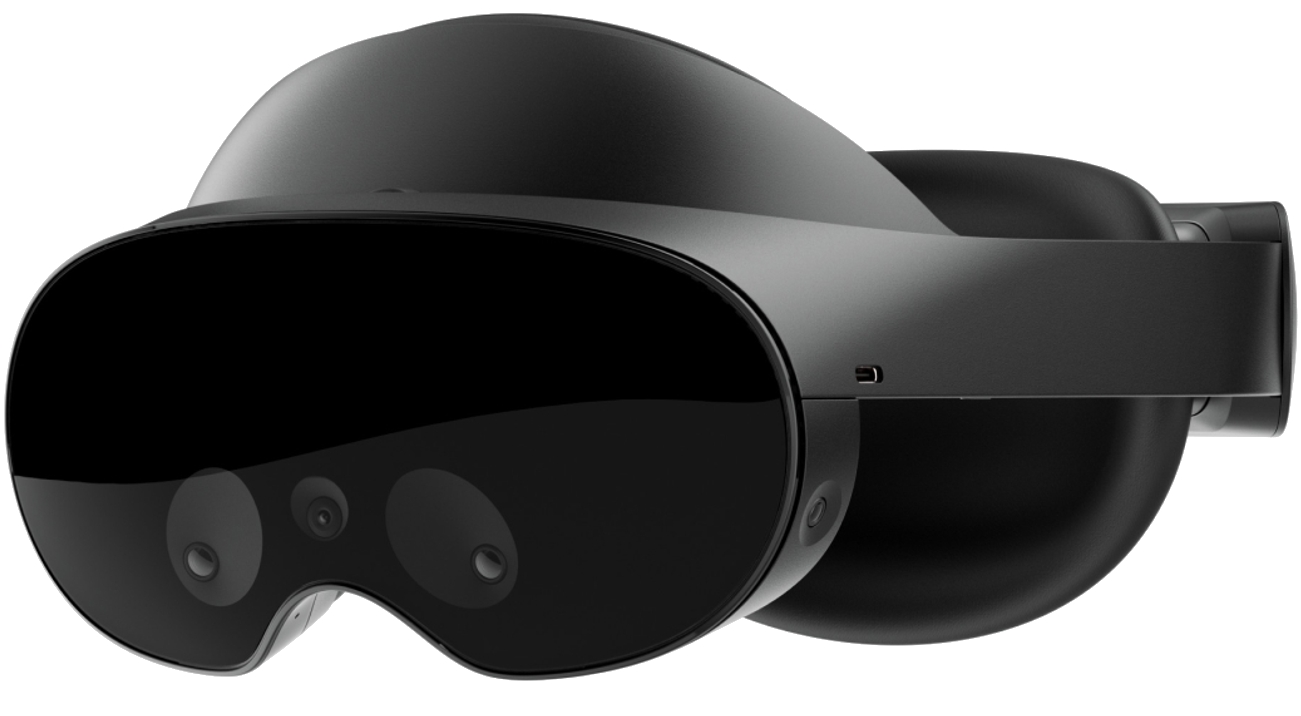
\includegraphics[width=2cm]{data/meta_quest.png}
    %                 };
    %             }
    %         }
    %         \only<7-11>{
    %             \node[align=center] at (0, -0.5) {
    %                 \textcolor{hiddencolour}{The role of neuroimaging beyond }T1-weighted MRI \textcolor{hiddencolour}{in the}\\\textcolor{hiddencolour}{diagnosis and prediction of neuropsychiatric disorders}
    %             };
    %             \onslide<8->{
    %                 \node[inner sep=0pt, label=below:{\labelsize{Bert from FreeSurfer 7.3}}] at (-3, -3.5) {
    %                     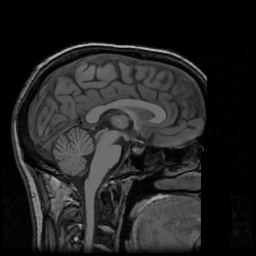
\includegraphics[width=3cm]{data/bert_sagittal.png}
    %                 };
    %             }
    %             \only<10>{
    %                 \node[] at (2, -4.2) {
    %                     \usebox{\modalities}
    %                 };
    %             }
    %             \only<11>{
    %                 \node[] at (2, -4.2) {
    %                     \usebox{\colouredmodalities}
    %                 };
    %             }
    %         }
    %         \only<12-16>{
    %             \def\nodefont{\footnotesize}
    %             \node[align=center] at (0, -0.5) {
    %                 \textcolor{hiddencolour}{The role of neuroimaging beyond T1-weighted MRI in the}\\\textcolor{hiddencolour}{diagnosis and prediction of }neuropsychiatric disorders
    %             };
    %             \onslide<13->{
    %                 \node[align=center, font=\nodefont] at (-2, -2) {
    %                     Alzheimer's disease and other\\causes of dementia
    %                 };
    %                 \node[align=center, font=\nodefont] at (-2.8, -2.8) {
    %                     Multiple Sclerosis
    %                 };
    %                 \node[align=center, font=\nodefont] at (-1.3, -3.2) {
    %                     Parkinson's Disease
    %                 };
    %             }

    %             \onslide<14->{
    %                 \node[align=center, font=\nodefont] at (1.9, -2.2) {
    %                     Bipolar Disorder
    %                 };
    %                 \node[align=center, font=\nodefont] at (1.6, -2.6) {
    %                     Schizophrenia
    %                 };
    %                 \node[align=center, font=\nodefont] at (2.8, -3.3) {
    %                     Depressive disorders
    %                 };
    %             }
    %             \onslide<15->{
    %                 \draw[stealth-stealth] (-4, -4) -- (4, -4);
    %             }
    %             \only<15>{
    %                 \node[anchor=east] at (-4, -4) {
    %                     \small{More}
    %                 };
    %                 \node[anchor=west] at (4, -4) {
    %                     \small{Less}
    %                 };
    %                 \node[anchor=north, font=\small] at (0, -4.1) {
    %                     Knowledge about neuropathological basis
    %                 };
    %             }
    %             \only<16>{
    %                 \node[anchor=east] at (-4, -4) {
    %                     \small{Less}
    %                 };
    %                 \node[anchor=west] at (4, -4) {
    %                     \small{More}
    %                 };
    %                 \node[anchor=north, font=\small] at (0, -4.1) {
    %                     Importance of psychopathology
    %                 };
    %             }
    %         }
    %         \onslide<17->{
    %             \node[align=center] at (0, -0.5) {
    %                 \textcolor{hiddencolour}{The role of neuroimaging beyond T1-weighted MRI in the}\\diagnosis and prediction \textcolor{hiddencolour}{of neuropsychiatric disorders}
    %             };
    %             \only<18>{
    %                 \node[label=below:{\scriptsize{Generated by DALL-E 3}}] at (0, -4.2) {
    %                     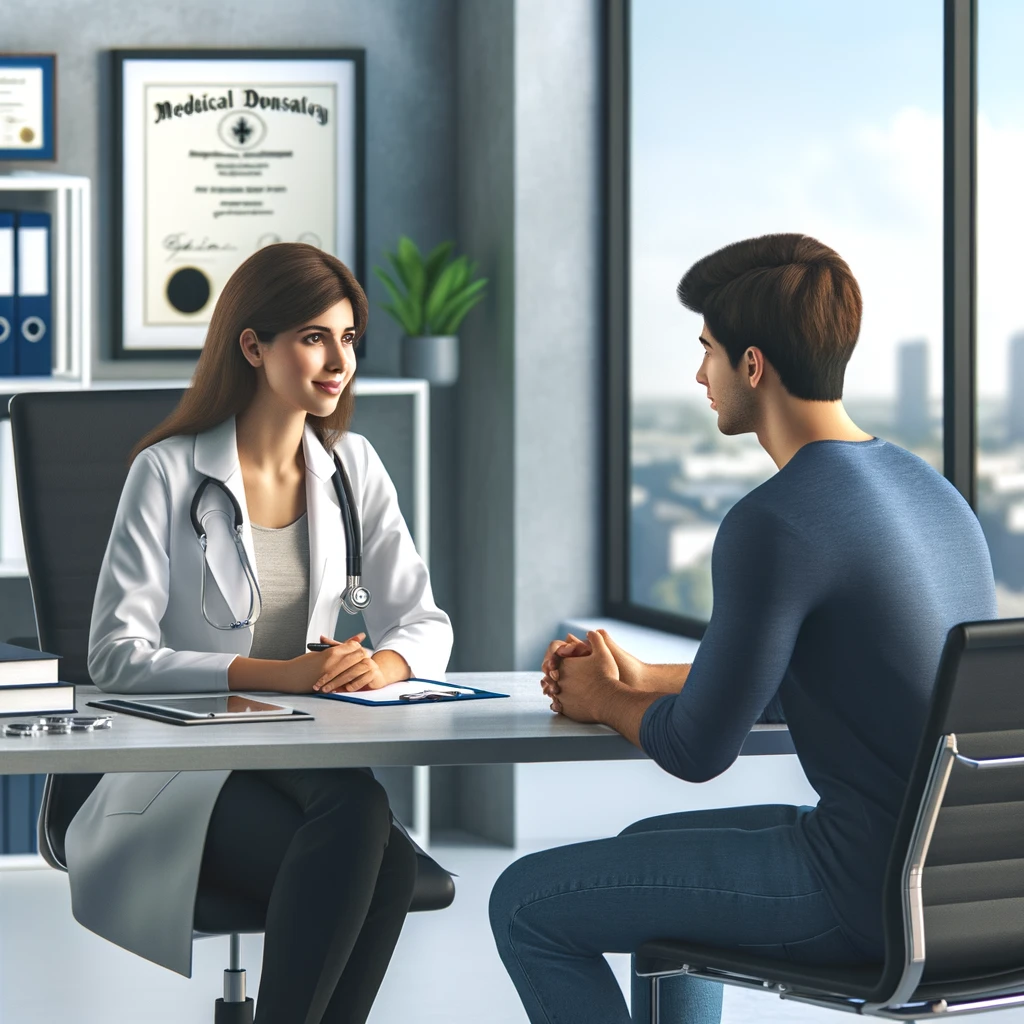
\includegraphics[width=5cm]{data/medical_consultancy.png}
    %                 };
    %             };
    %             \only<19>{
    %                 \node[label=below:{\labelsize{Vogel \& Black (2024)}}, inner sep=0pt, draw=black] at (0, -3.5) {
    %                     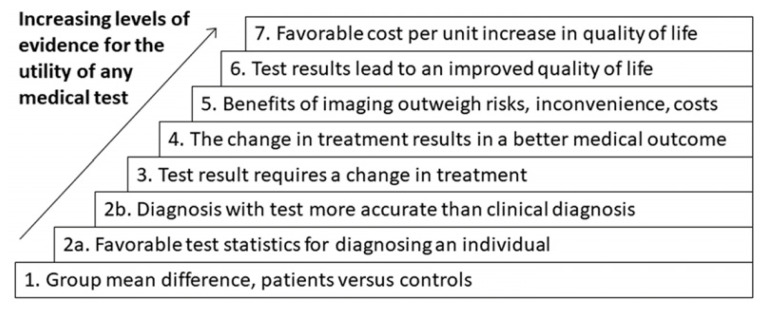
\includegraphics[width=7cm]{data/diagnostic_predictions.jpeg}
    %                 };

    %                 \node[font=\tiny, anchor=south,align=center, inner sep=1pt] (psych-citation) at (0, -7.65) {
    %                     Vogel, A. C., \& Black, K. J. (2024). Brain Imaging in Routine Psychiatric Practice. Missouri Medicine, 121(1), 37
    %                 };

    %             }
    %             \onslide<20->{
    %                 \only<20>{
    %                     \node[inner sep=0pt] at (-2.8, -4)  {
    %                         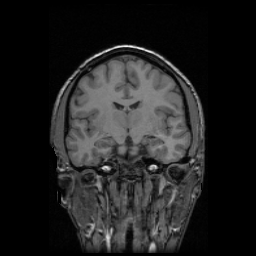
\includegraphics[width=3.5cm]{data/bert_coronal.png}
    %                     };
    %                 }
    %                 \onslide<21->{
    %                     \node[inner sep=0pt] (bert) at (-2.8, -4) {
    %                         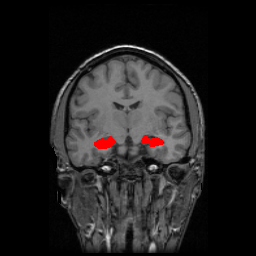
\includegraphics[width=3.5cm]{data/bert_coronal_marked.png}
    %                     };

    %                 }
    %                 \only<22-23>{
    %                     \node[] at (3.4, -4.3) {
    %                         \scriptsize{Data from ADNI}
    %                     };
    %                     \node[font=\tiny, align=center, anchor=south] at (0, -7.75) {
    %                         Jack Jr, C. R., Bernstein, M. A., Fox, N. C., Thompson, P., Alexander, G., Harvey, D., ... \& Weiner, M. W. (2008). The Alzheimer's disease\\neuroimaging initiative (ADNI): MRI methods. Journal of Magnetic Resonance Imaging: An Official Journal of the International\\Society for Magnetic Resonance in Medicine, 27(4), 685-691
    %                     };
    %                 }
    %                 \only<22>{
    %                     \node[anchor=south] at (3.66, -4.15) {
    %                         \usebox{\casehippo}
    %                     };
    %                 }
    %                 \only<23,24>{
    %                     \node[anchor=south] at (3.66, -4.15) {
    %                         \usebox{\hippo}
    %                     };
    %                 }
    %                 \only<24>{
    %                     \node[] at (3, -5.5) {
    %                         \usebox{\hippoauc}
    %                     };
    %                 }
    %                 \onslide<25->{
    %                     \node[align=center,draw=gray,fill=gray!20, inner sep=5pt] (model) at (1.2, -4) {Predictive\\model};
    %                     \node[align=center,text depth=0, anchor=west] (patient) at (3.3, -3.6) {Patient};
    %                     \node[align=center,text depth=0, anchor=west] (control) at (3.3, -4.4) {Control};

    %                     \draw[-stealth, thick] (bert) -- (model);
    %                     \draw[-stealth, thick] (model.east) -- (patient.west);
    %                     \draw[-stealth, thick] (model.east) -- (control.west);
    %                 }
    %             }
    %         }
    %     \end{tikzpicture}
    % \end{frame}
    \section{\large{Neuroimaging modalities for diagnostic predictions}}

    \begin{frame}{Approach}
        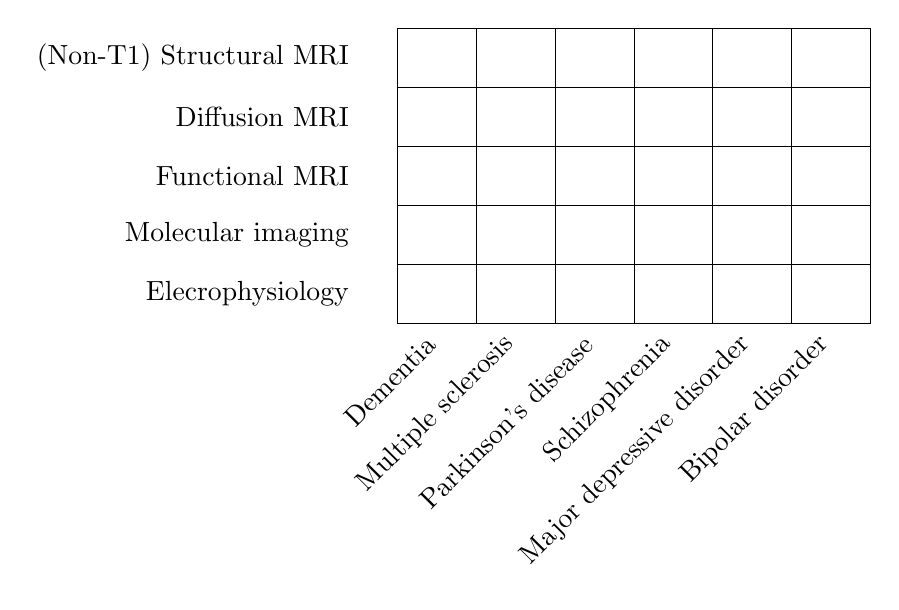
\begin{tikzpicture}
            \node[anchor=east] at (0, 0) {
                (Non-T1) Structural MRI
            };
            \node[anchor=east] at (0, -0.75) {
                Diffusion MRI
            };
            \node[anchor=east] at (0, -1.5) {
                Functional MRI
            };
            \node[anchor=east] at (0, -2.25) {
                Molecular imaging
            };
            \node[anchor=east] at (0, -3) {
                Elecrophysiology
            };

            \onslide<2->{
                \node[anchor=east,rotate=45] at (1, -3.5) {Dementia};
                \node[anchor=east,rotate=45] at (2, -3.5) {Multiple sclerosis};
                \node[anchor=east,rotate=45] at (3, -3.5) {Parkinson's disease};
                \node[anchor=east,rotate=45] at (4, -3.5) {Schizophrenia};
                \node[anchor=east,rotate=45] at (5, -3.5) {Major depressive disorder};
                \node[anchor=east,rotate=45] at (6, -3.5) {Bipolar disorder};
            }

            \onslide<3->{
                \draw[] (0.5, 0.375) -- (0.5, -3.375);
                \draw[] (1.5, 0.375) -- (1.5, -3.375);
                \draw[] (2.5, 0.375) -- (2.5, -3.375);
                \draw[] (3.5, 0.375) -- (3.5, -3.375);
                \draw[] (4.5, 0.375) -- (4.5, -3.375);
                \draw[] (5.5, 0.375) -- (5.5, -3.375);
                \draw[] (6.5, 0.375) -- (6.5, -3.375);

                \draw[] (0.5, 0.375) -- (6.5, 0.375);
                \draw[] (0.5, -0.375) -- (6.5, -0.375);
                \draw[] (0.5, -1.125) -- (6.5, -1.125);
                \draw[] (0.5, -1.875) -- (6.5, -1.875);
                \draw[] (0.5, -2.625) -- (6.5, -2.625);
                \draw[] (0.5, -3.375) -- (6.5, -3.375);
            }
        \end{tikzpicture}
    \end{frame}

    \begin{frame}{Data}
        \begin{tikzpicture}
            \only<1-5>{
                \node[draw=black,inner sep=2pt] (wolfers) at (0, 0) {
                    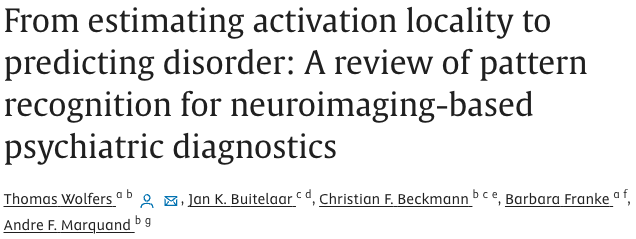
\includegraphics[width=4cm]{data/wolfers_2015.png}
                };
                \onslide<2->{
                    \node[draw=black,inner sep=2pt, anchor=north] (arbabshirani) at ($ (wolfers.south) - (0, 0.2) $) {
                        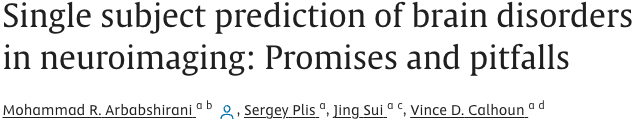
\includegraphics[width=4cm]{data/arbabshirani_2017.png}
                    };
                }
                \onslide<3->{
                    \node[draw=black,inner sep=2pt, anchor=north] (rashid) at ($ (arbabshirani.south) - (0, 0.2) $) {
                        
\includegraphics[width=4cm]{data/rashid_2020.png}
                    };
                }
                \onslide<4->{
                    \node[draw=black,inner sep=2pt, anchor=north] (quaak) at ($ (rashid.south) - (0, 0.2) $) {
                        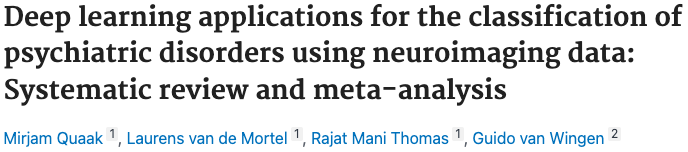
\includegraphics[width=4cm]{data/quaak_2021.png}
                    };
                }
                \onslide<5->{
                    \node[draw=black,inner sep=2pt, anchor=north] at  ($ (quaak.south) - (0, 0.2) $) {
                        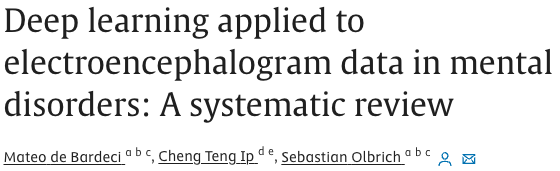
\includegraphics[width=4cm]{data/bardeci_2021.png}
                    };
                }
            }
            \only<6-8>{
                \node[draw=black,inner sep=2pt] (ebrahim) at (0, -0.5) {
                    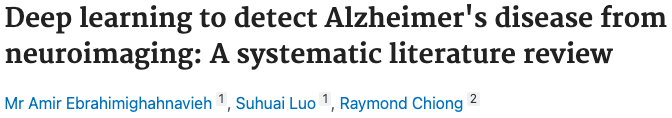
\includegraphics[width=4cm]{data/ebrahimighahnavieh_2020.png}
                };
                \onslide<7->{
                    \node[draw=black,inner sep=2pt, anchor=north] (mirzaei) at ($ (ebrahim.south) - (0, 0.2) $) {
                        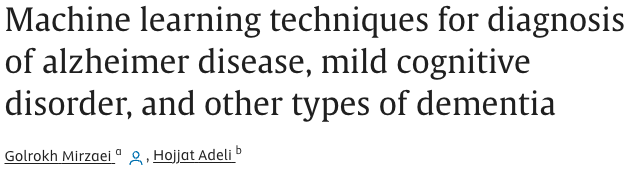
\includegraphics[width=4cm]{data/mirzaei_2022.png}
                    };
                }
                \onslide<8->{
                    \node[draw=black,inner sep=2pt, anchor=north] (fathi) at ($ (mirzaei.south) - (0, 0.2) $) {
                        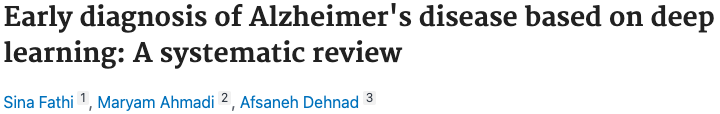
\includegraphics[width=4cm]{data/fathi_2022.png}
                    };
                }
            }
            \only<9,10>{
                \node[draw=black,inner sep=2pt] (shoeibi) at (0, -1.2) {
                    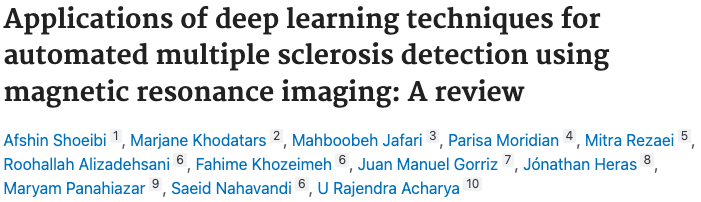
\includegraphics[width=4cm]{data/shoeibi_2021.png}
                };
                \onslide<10->{
                    \node[draw=black,inner sep=2pt, anchor=north] (aslam) at ($ (shoeibi.south) - (0, 0.2) $) {
                        
\includegraphics[width=4cm]{data/aslam_2022.png}
                    };
                }
            }
            \only<11>{
                \node[draw=black,inner sep=2pt] (aggarwal) at (0, -2) {
                    
\includegraphics[width=4cm]{data/aggarwal_2023.png}
                };
            }
            \only<12,13>{
                \node[draw=black,inner sep=2pt] (filippis) at (0, -1.2) {
                    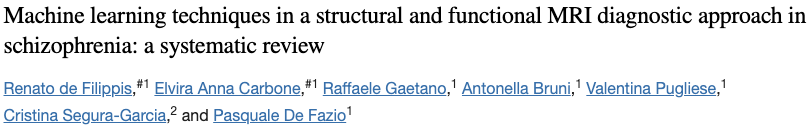
\includegraphics[width=4cm]{data/filippis_2019.png}
                };
                \onslide<13->{
                    \node[draw=black,inner sep=2pt, anchor=north] (verma) at ($ (filippis.south) - (0, 0.2) $) {
                        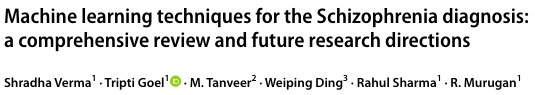
\includegraphics[width=4cm]{data/verma_2023.png}
                    };
                }
            }
            \only<14>{
                \node[draw=black,inner sep=2pt] (aggarwal) at (0, -2) {
                    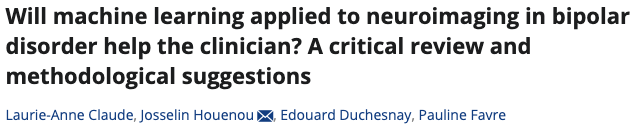
\includegraphics[width=4cm]{data/claude_2020.png}
                };
            }
        \end{tikzpicture}
    \end{frame}

    \newsavebox{\ttwostudies}
    \sbox{\ttwostudies}{%
        \begin{tikzpicture}
            \begin{axis}[
                ymin=50,
                ymax=100,
                xtick={2016, 2018, 2020, 2022},
                xticklabels={2016, 2018, 2020, 2022},
                xlabel=Year,
                ylabel=Accuracy,
                width=5cm,
                height=5cm,
                every tick label/.append style={font=\footnotesize},
                xtick pos=bottom,
                ytick pos=left,
                clip=false,
                xmin=2015.5,
                xmax=2022.5
            ]
                \addplot[
                    only marks,
                    scatter,
                    scatter/classes={
                        MS={mark=*,color1},
                        PD={mark=*,color4}
                    },
                    scatter src=explicit symbolic,
                    visualization depends on={ln(\thisrow{sample}*0.5) \as \perpointmarksize},
                    scatter/@pre marker code/.append style={
                        /tikz/mark size=\perpointmarksize
                    },
                    opacity=0.75
                ] table [
                    x=year,
                    y=accuracy,
                    col sep=comma,
                    meta=diagnosis
                ] {data/t2_studies.csv};
            \end{axis}
        \end{tikzpicture}
    }

    \begin{frame}{Other structural MRI modalities (T2, FLAIR)}
        \centering
        \begin{tikzpicture}
            \def\labelsize{\footnotesize}

            \node[draw=black] at (0, 0) {};
            \node[draw=black] at (10, -7) {};
            \onslide<1->{
                \node[anchor=west] (t1) at (0, -3.5) {
                    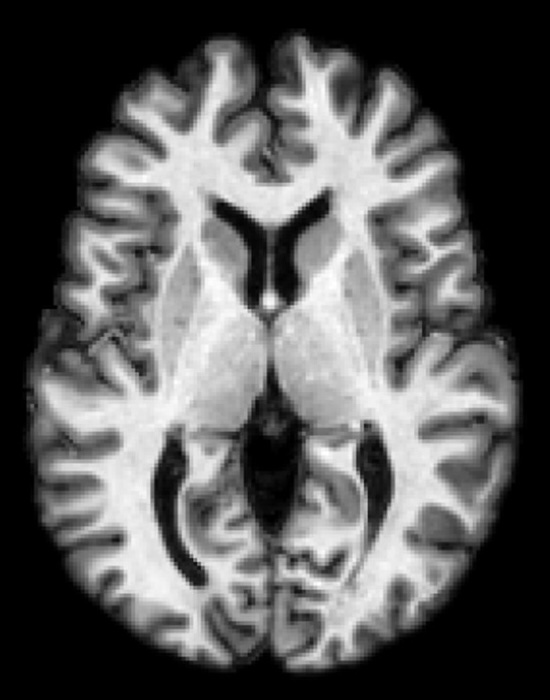
\includegraphics[
                        height=1.7cm
                    ]{data/t1.jpg}
                };
                \node[anchor=south, inner sep=0pt] at (t1.north) {\labelsize{T1}};
            }
            \onslide<2->{
                \node[anchor=west] (t2) at ($ (t1.east) - (0.35, 0) $) {
                    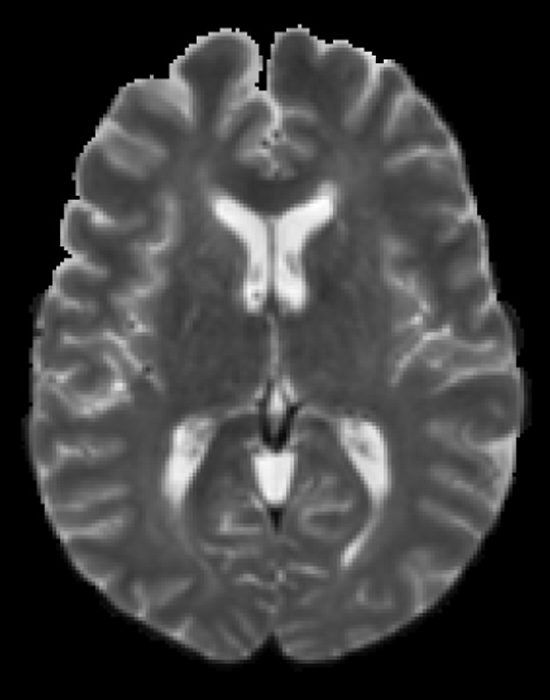
\includegraphics[
                        height=1.7cm
                    ]{data/t2.jpg}
                };
                \node[anchor=south, inner sep=0pt] at (t2.north) {\labelsize{T2}};
            }
            \onslide<3->{
                \node[anchor=west] (flair) at ($ (t2.east) - (0.35, 0) $) {
                    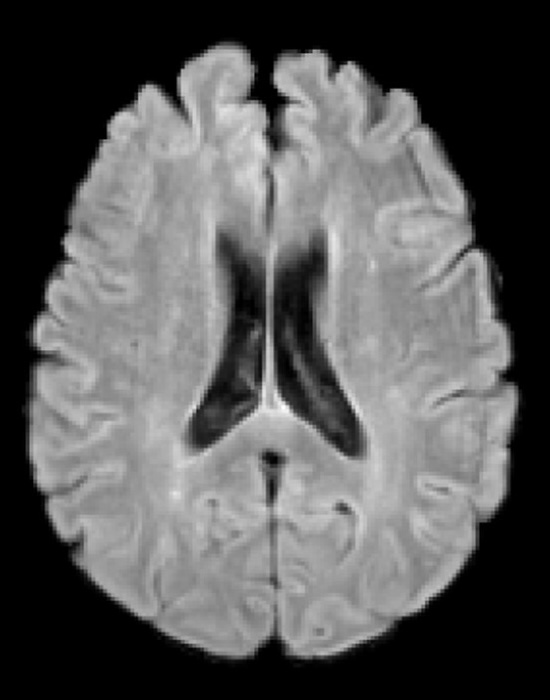
\includegraphics[
                        height=1.7cm
                    ]{data/flair.jpg}
                };
                \node[anchor=south, inner sep=0pt] at (flair.north) {\labelsize{FLAIR}};
                \node[anchor=north] at ($ (t2.south) - (0, -0.15) $) {\scriptsize{Adapted from Shoeibi et al., 2021}};
                \only<3>{
                    \node[font=\tiny, anchor=south,align=center, inner sep=1pt] (ms-citation) at (5, -7.5) {
                        Shoeibi, A., Khodatars, M., Jafari, M., Moridian, P., Rezaei, M., Alizadehsani, R., ... \& Acharya, U. R. (2021). Applications of deep learning\\techniques for automated multiple sclerosis detection using magnetic resonance imaging: A review. Computers in Biology and\\Medicine, 136, 104697
                    };
                }
            }
            \only<4>{
                \node[] at (7.6, -3.2) {
                    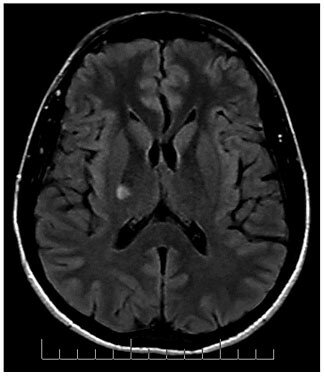
\includegraphics[width=4cm]{data/flair_lesion.jpeg}
                };
            }
            \only<5>{
                \node[] at (7.6, -3.2) {
                    \usebox{\ttwostudies}
                };
            };
            \only<6>{
                \node[label=below:\scriptsize{De Angelis et al., 2019}, inner sep=0pt, draw=black] at (7.6, -3.2) {
                    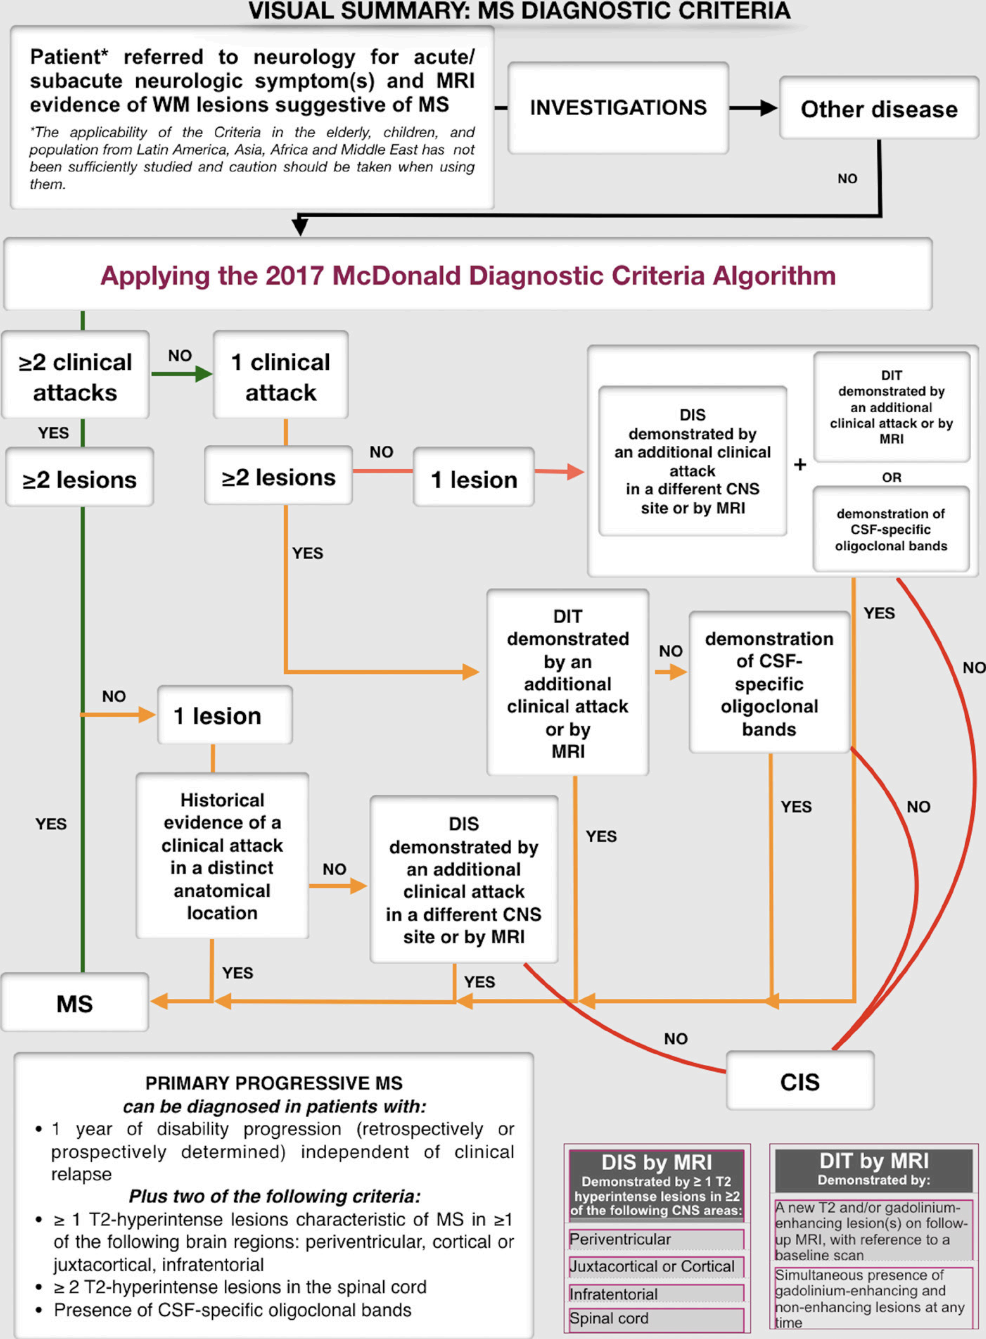
\includegraphics[width=4.5cm]{data/ms_criteria.png}
                };
                \node[font=\tiny, anchor=south,align=center, inner sep=1pt] (ms-citation) at (5, -7.65) {
                    De Angelis, F., Brownlee, W. J., Chard, D. T., \& Trip, S. A. (2019). New MS diagnostic criteria in practice. Practical Neurology, 19(1), 64-67
                };
            }
            \only<7>{
                \node[] at (7.6, -3.2) {
                    T2 use-case in PD: WML/Motoric problems
                };
            }
            \only<8>{
                \node[] at (7.6, -3.2) {
                    T2 use-case in dementia: WML/Subtyping
                };
            }
        \end{tikzpicture}
    \end{frame}

    \newsavebox{\dmristudies}
    \sbox{\dmristudies}{%
        \begin{tikzpicture}
            \begin{axis}[
                ymin=50,
                ymax=100,
                xlabel=Year,
                ylabel=Accuracy,
                width=5cm,
                height=5cm,
                every tick label/.append style={font=\footnotesize},
                xtick pos=bottom,
                ytick pos=left,
            ]
                \addplot[
                    only marks,
                    scatter,
                    scatter/classes={
                        AD={mark=*,color1},
                        SCZ={mark=*,color3},
                        MDD={mark=*,color5},
                        BP={mark=*,color7}
                    },
                    scatter src=explicit symbolic,
                    visualization depends on={ln(\thisrow{sample}*0.5) \as \perpointmarksize},
                    scatter/@pre marker code/.append style={
                        /tikz/mark size=\perpointmarksize
                    },
                    opacity=0.75
                ] table [
                    x=year,
                    y=accuracy,
                    col sep=comma,
                    meta=diagnosis
                ] {data/dMRI_studies.csv};
            \end{axis}
        \end{tikzpicture}
    }

    \begin{frame}{Diffusion MRI (DTI?)}
        \begin{tikzpicture}
            \node[draw=black] at (0, 0) {};
            \node[draw=black] at (10, -7) {};

            \onslide<1->{
                \node[] at (2, -3.5) {
                    Explanation of DTI
                };
            }
            \only<2>{
                \node[] at (7.6, -3.2) {
                    \usebox{\dmristudies}
                };
            };
            \only<3>{
                \node[] at (7.6, -3.2) {
                    Lack of prediction studies
                };
            }
            \only<4>{
                \node[] at (7.6, -3.2) {
                    DTI use case 1
                };
            }
            \only<5>{
                \node[] at (7.6, -3.2) {
                    DTI use case 2
                };
            }
        \end{tikzpicture}
    \end{frame}

    \begin{frame}{Molecular imaging (PET/SPECT)}
        % https://www.ncbi.nlm.nih.gov/pmc/articles/PMC9181385/#B45-ijms-23-06079
        \begin{tikzpicture}
            \node[draw=black] at (0, 0) {};
            \node[draw=black] at (10, -7) {};

            \onslide<1->{
                \node[] at (2, -3.5) {
                    Explanation of PET
                };
            }
            \only<2>{
                \node[] at (7.6, -3.2) {
                    PET/SPECT in meta-analysis
                };
            };
            \only<3>{
                \node[] at (7.6, -3.2) {
                    PET in AD
                };
            }
            \only<4>{
                \node[] at (7.6, -3.2) {
                    SPECT in PD
                };
            }
            \only<5>{
                \node[] at (7.6, -3.2) {
                    Mental disorders?
                };
            }
        \end{tikzpicture}
    \end{frame}

    \newsavebox{\fmristudies}
    \sbox{\fmristudies}{%
        \begin{tikzpicture}
            \begin{axis}[
                ymin=50,
                ymax=100,
                xlabel=Year,
                ylabel=Accuracy,
                width=5cm,
                height=5cm,
                every tick label/.append style={font=\footnotesize},
                xtick pos=bottom,
                ytick pos=left,
            ]
                \addplot[
                    only marks,
                    scatter,
                    scatter/classes={
                        AD={mark=*,color1},
                        SCZ={mark=*,color3},
                        MDD={mark=*,color5},
                        BP={mark=*,color7}
                    },
                    scatter src=explicit symbolic,
                    visualization depends on={ln(\thisrow{sample}*0.5) \as \perpointmarksize},
                    scatter/@pre marker code/.append style={
                        /tikz/mark size=\perpointmarksize
                    },
                    opacity=0.75
                ] table [
                    x=year,
                    y=accuracy,
                    col sep=comma,
                    meta=diagnosis
                ] {data/fMRI_studies.csv};
            \end{axis}
        \end{tikzpicture}
    }

    \begin{frame}{Functional Magnetic Resonance Imaging (fMRI)}
        \begin{tikzpicture}
            \node[draw=black] at (0, 0) {};
            \node[draw=black] at (10, -7) {};

            \onslide<1->{
                \node[] at (2, -3.5) {
                    Explanation of fMRI
                };
            }
            \only<2>{
                \node[] at (7.6, -3.2) {
                    Task vs rest
                };
            };
            \only<3>{
                \node[] at (7.6, -3.2) {
                    \usebox{\fmristudies}
                };
            }
            \only<4>{
                \node[] at (7.6, -3.2) {
                    fMRI use-case 1
                };
            }
            \only<5>{
                \node[] at (7.6, -3.2) {
                    fMRI use-case 2
                };
            }
        \end{tikzpicture}
    \end{frame}

    \begin{frame}{Elecrophysiological mapping (EEG/MEG)}
    \end{frame}

    \begin{frame}{Alzheimer's disease}
        \centering
        \begin{itemize}
            \item Pathological changes are apparent in a variety of neuroimaging modalities, to a level which can support individual diagnostics.
            \item
        \end{itemize}
        \begin{tikzpicture}
            %https://www.ncbi.nlm.nih.gov/pmc/articles/PMC9181385/
            \node[inner sep=0pt, draw=black] at (0, 0) {
                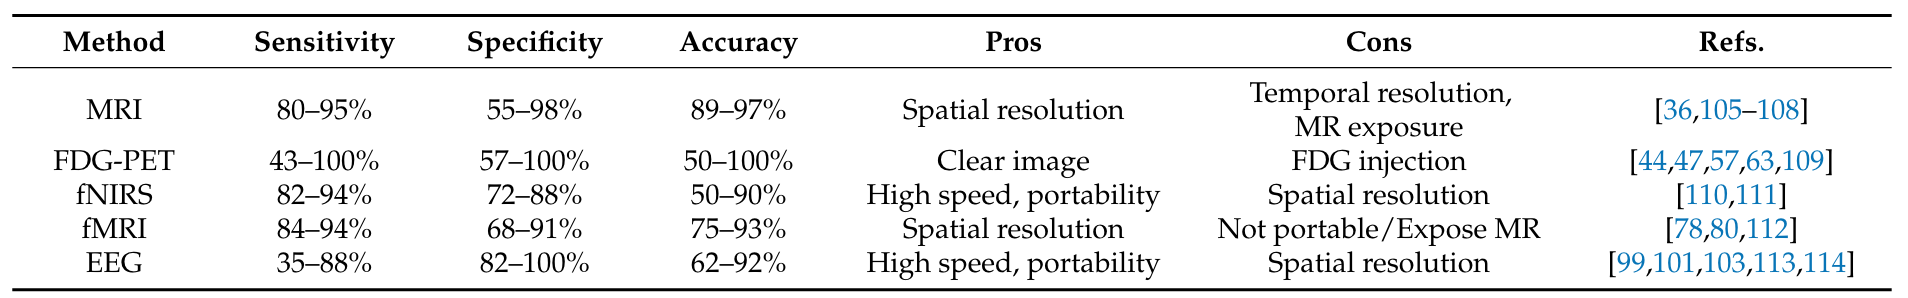
\includegraphics[width=9cm]{data/AD_modalities.png}
            };
        \end{tikzpicture}
    \end{frame}
    \begin{frame}{Multiple sclerosis}
        \begin{itemize}
            \item Lesions apparent in T2-weighted and FLAIR images are used clinically to support diagnostics.
            \item DTI reveals group-wise differences also in apparently healthy white matter.
            \item A stereotypical trajectory that has been observed in patients using fMRI is heightened activation up until a point where it is no longer possible to compensate for structural damage, after which the activation generally resides.
        \end{itemize}
    \end{frame}
    \begin{frame}{Parkinson's disease}
        % https://www.ncbi.nlm.nih.gov/pmc/articles/PMC6280219/
        % https://link.springer.com/article/10.1007/s12559-023-10175-y
        \begin{itemize}
            \item DTI has been shown useful for classifying patient subtypes and correlates with motor and cognitive function in PD patients.
            \item fMRI has been shown useful for differentiating patient subtypes, supporting the notion of PD subtypes as network models.
            \item PET imaging can be used to reveal subtypes
        \end{itemize}
    \end{frame}

    \begin{frame}{Bipolar disorder}
        \begin{tikzpicture}
            \only<1>{
                % https://pubmed.ncbi.nlm.nih.gov/32108409/
                \node[inner sep=0pt, draw=black] at (0, 0) {
                    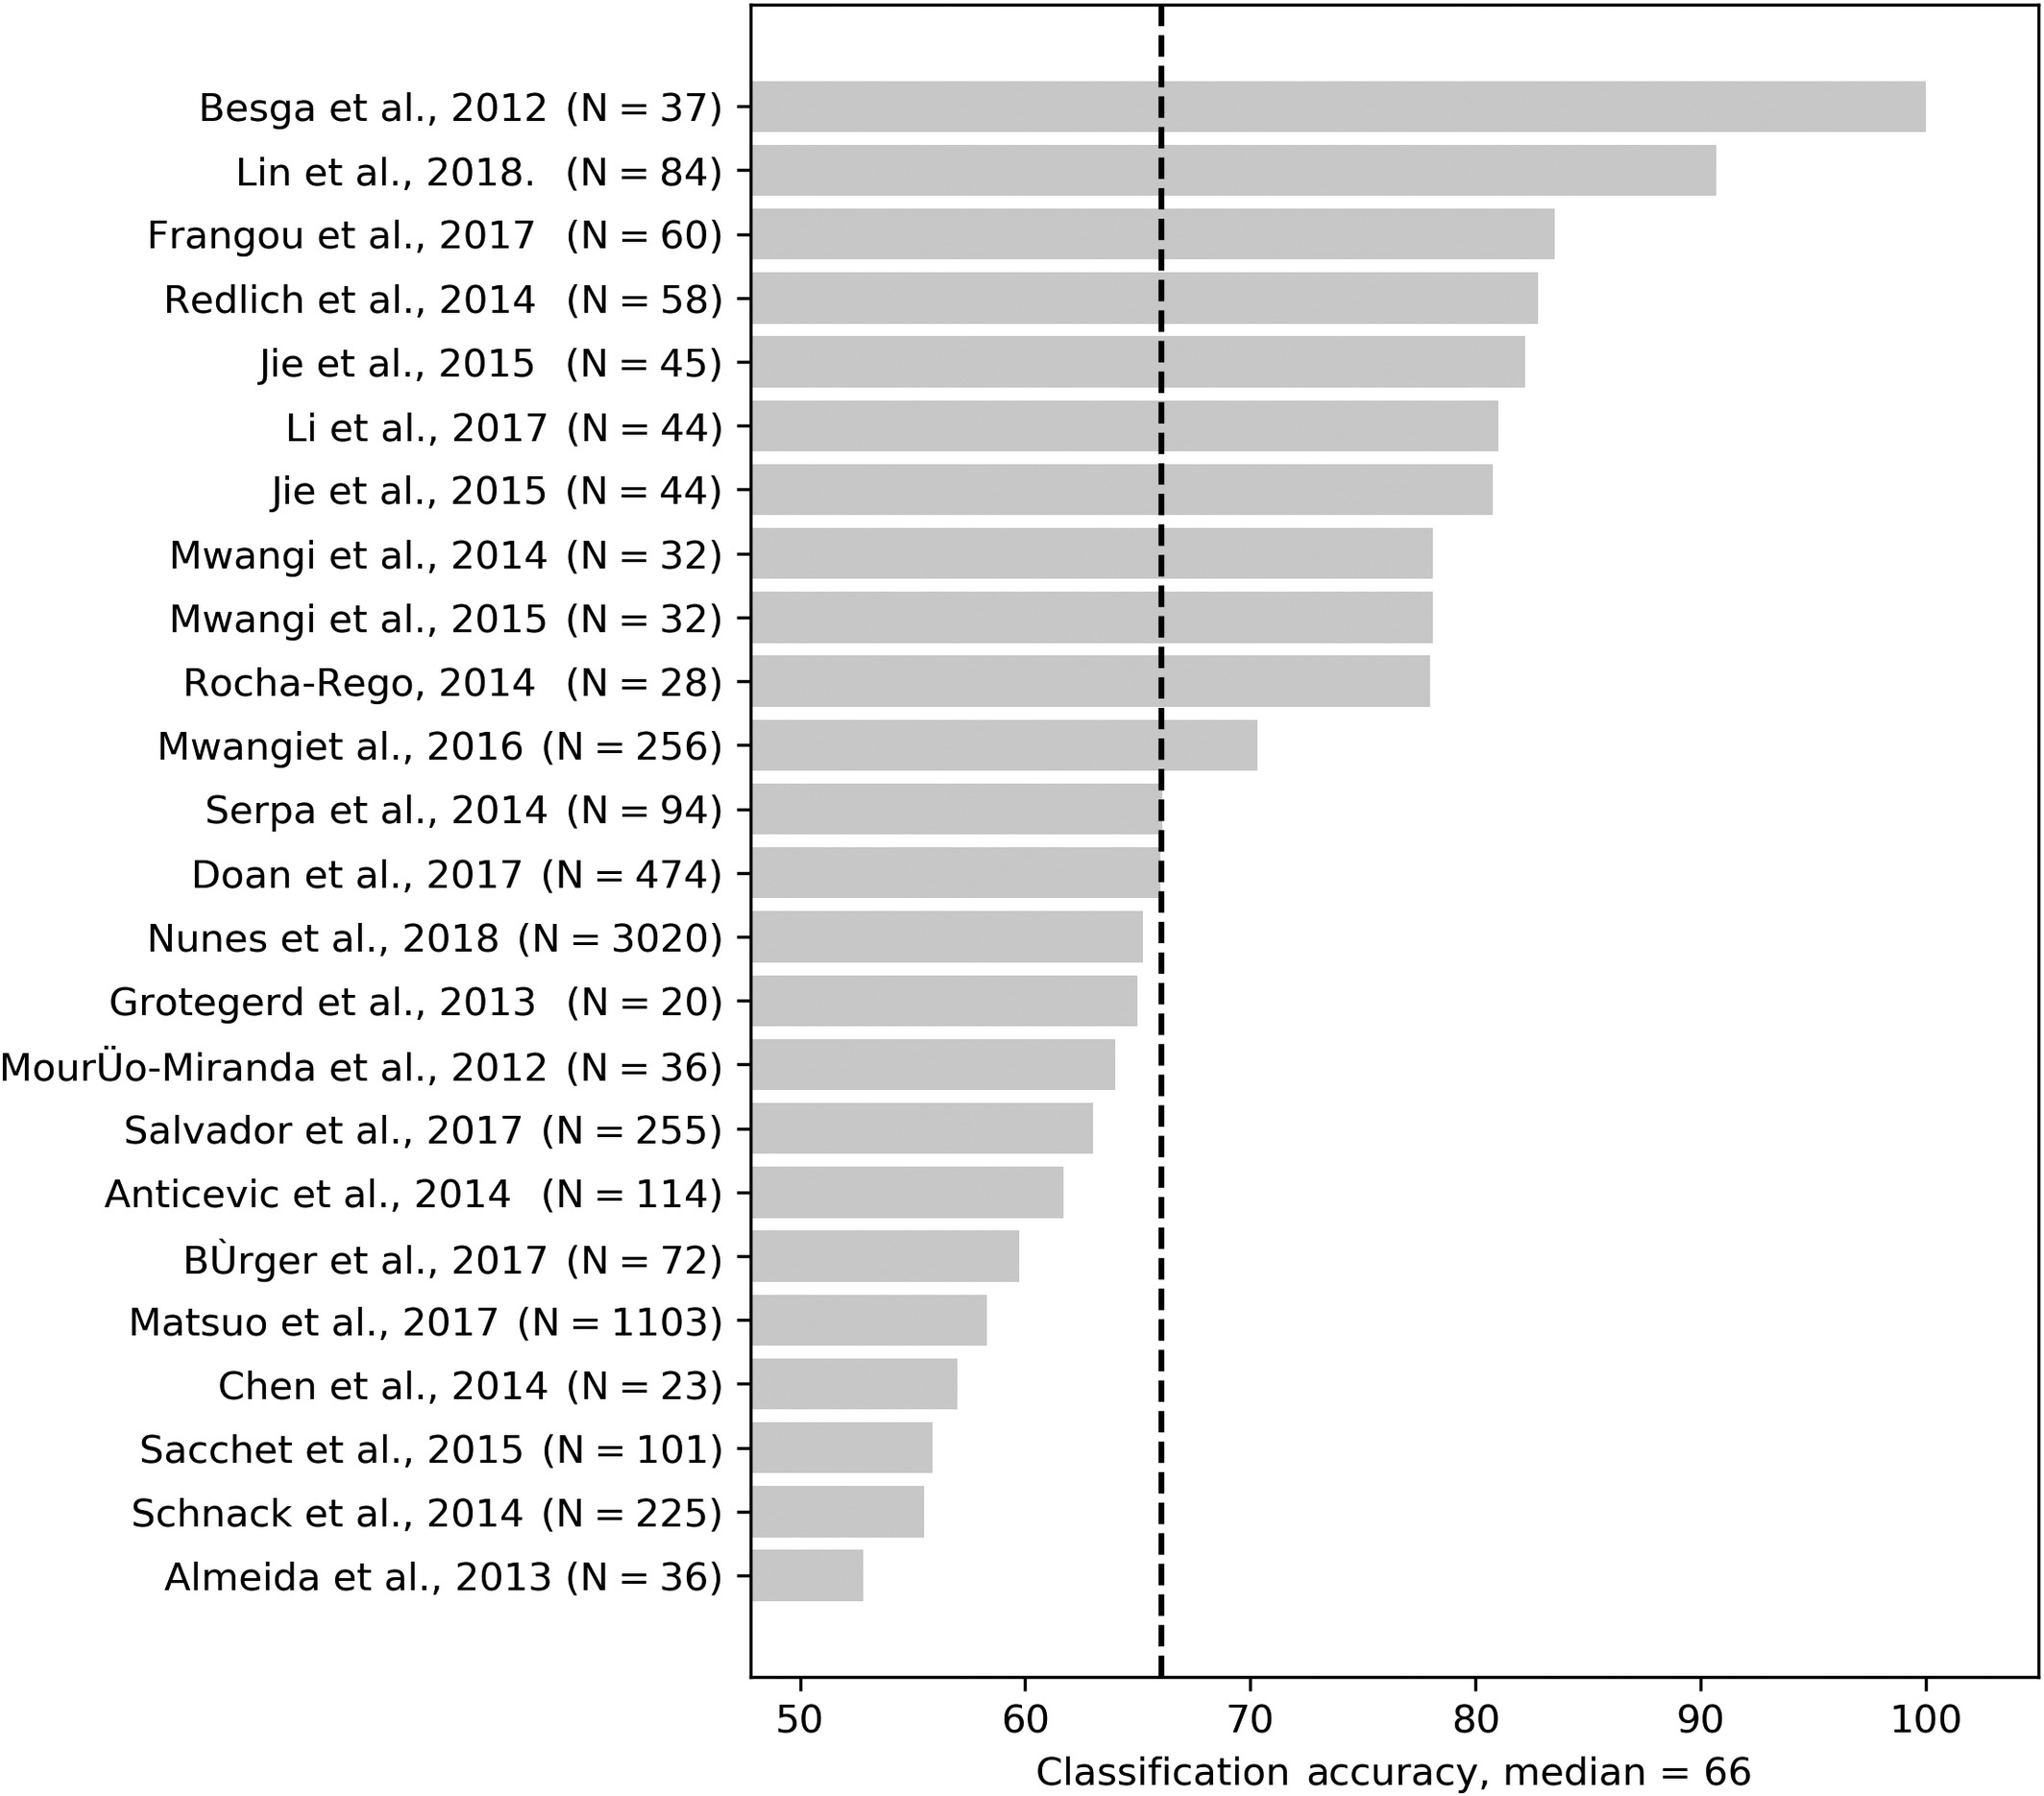
\includegraphics[width=8cm]{data/bp_accuracies.jpeg}
                };
            }
            \only<2>{
                % https://academic.oup.com/cercor/article/29/1/202/4653730?login=false
                \node[inner sep=0pt, draw=black] at (0, 0) {
                    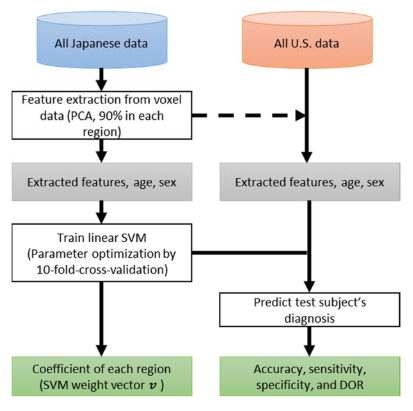
\includegraphics[width=6cm]{data/bp_generalization.png}
                };
            }
        \end{tikzpicture}
    \end{frame}

    \begin{frame}{Schizophrenia}
    \end{frame}

    \begin{frame}{Major depressive disorder}
    \end{frame}

    % \section{The future of neuroimaging-based prediction}

    % \newsavebox{\accuracyplots}
    % \sbox{\accuracyplots}{%
    %     \begin{tikzpicture}
    %         \begin{axis}[
    %             boxplot/draw direction = y,
    %             width=10cm,
    %             height=7cm,
    %             xmin=0.4,
    %             xmax=6.6,
    %             ymin=50,
    %             ymax=100,
    %             xtick={1,2,3,4,5,6},
    %             xticklabels={DEM,MS,PD,SCZ,MDD,BP},
    %             ylabel=Accuracy,
    %             axis y line*=left,
    %             xlabel=Diagnosis,
    %             axis x line*=bottom,
    %             clip=false,
    %             xtick style={draw=none},
    %             ymajorgrids=true,
    %             ytick style={draw=none},
    %         ]
    %         % DEM
    %         \addplot[] coordinates { (0.595, 92.5) (1.405, 92.5) };
    %         \addplot[] coordinates { (1.595, 93.4) (2.405, 93.4) };
    %         \addplot[] coordinates { (2.595, 95.15) (3.405, 95.15) };
    %         \addplot[] coordinates { (3.595, 81.8) (4.405, 81.8) };
    %         \addplot[] coordinates { (4.595, 85) (5.405, 85) };
    %         \addplot[] coordinates { (5.595, 68.2) (6.405, 68.2) };
    %         \node[anchor=south] at (axis cs: 1, 92.5) {92.5\%};
    %         \node[anchor=south] at (axis cs:2, 93.4) {93.4\%};
    %         \node[anchor=south] at (axis cs:3, 95.15) {95.15\%};
    %         \node[anchor=south] at (axis cs:4, 81.8) {81.8\%};
    %         \node[anchor=south] at (axis cs:5, 85) {85\%};
    %         \node[anchor=south] at (axis cs:6, 68.2) {68.2\%};
    %         \end{axis}
    %     \end{tikzpicture}
    % }

    % \newsavebox{\boxplots}
    % \sbox{\boxplots}{%
    %     \begin{tikzpicture}
    %         \begin{axis}[
    %             boxplot/draw direction = y,
    %             width=10cm,
    %             height=7cm,
    %             xmin=0.4,
    %             xmax=6.6,
    %             ymin=50,
    %             ymax=100,
    %             xtick={1,2,3,4,5,6},
    %             xticklabels={DEM,MS,PD,SCZ,MDD,BP},
    %             ylabel=Accuracy,
    %             axis y line*=left,
    %             xlabel=Diagnosis,
    %             axis x line*=bottom,
    %             clip=false,
    %             xtick style={draw=none},
    %             ymajorgrids=true,
    %             ytick style={draw=none},
    %         ]
    %         % DEM
    %         \addplot[red] coordinates { (0.595, 92.5) (1.405, 92.5) };
    %         \addplot+[
    %             boxplot prepared={
    %             median=92.5,
    %             upper quartile=97.25,
    %             lower quartile=88.94,
    %             upper whisker=100,
    %             lower whisker=76.46
    %             },
    %             draw=black,
    %             fill=color1,
    %             solid
    %         ] coordinates {};

    %         % MS
    %         \addplot+[
    %             boxplot prepared={
    %             median=93.4,
    %             upper quartile=98.26,
    %             lower quartile=87.9,
    %             upper whisker=100,
    %             lower whisker=72.36
    %             },
    %             draw=black,
    %             fill=color2,
    %             solid
    %         ] coordinates {};

    %         % PD
    %         \addplot+[
    %             boxplot prepared={
    %             median=95.15,
    %             upper quartile=97.07,
    %             lower quartile=89.15,
    %             upper whisker=100,
    %             lower whisker=77.26
    %             },
    %             draw=black,
    %             fill=color3,
    %             solid
    %         ] coordinates {};

    %         % SCZ
    %         \addplot+[
    %             boxplot prepared={
    %             median=81.8,
    %             upper quartile=90.28,
    %             lower quartile=75,
    %             upper whisker=100,
    %             lower whisker=62
    %             },
    %             draw=black,
    %             fill=color4,
    %             solid
    %         ] coordinates {};

    %         % MDD
    %         \addplot+[
    %             boxplot prepared={
    %             median=85,
    %             upper quartile=91.7,
    %             lower quartile=73,
    %             upper whisker=99,
    %             lower whisker=50.55
    %             },
    %             draw=black,
    %             fill=color5,
    %             solid
    %         ] coordinates {};

    %         % BP
    %         \addplot+[
    %             boxplot prepared={
    %             median=68.2,
    %             upper quartile=78.59,
    %             lower quartile=61.03,
    %             upper whisker=100,
    %             lower whisker=55.9
    %             },
    %             draw=black,
    %             fill=color6,
    %             solid
    %         ] coordinates {};
    %         \end{axis}
    %     \end{tikzpicture}
    % }

    % \newsavebox{\sizeplots}
    % \sbox{\sizeplots}{%
    %     \begin{tikzpicture}
    %         \begin{groupplot}[
    %             group style={
    %                 group size=3 by 2,
    %                 horizontal sep=0.25cm,
    %                 group name=plots,
    %                 vertical sep=1.35cm
    %             },
    %             height=3.9cm,
    %             width=4.4cm,
    %             ymin=50,
    %             ymax=100,
    %             ticklabel style = {font=\footnotesize},
    %             xmin=0,
    %             xlabel={\footnotesize{Size}},
    %             x label style={at={(axis description cs:0.5,-0.15)},anchor=north},
    %             y label style={at={(axis description cs:-0.15,.5)},anchor=south},
    %         ]
    %             \nextgroupplot[
    %                 ylabel={\footnotesize{Accuracy}},
    %                 ymajorgrids=true,
    %                 ytick style={draw=none},
    %                 xmax=4700
    %             ]
    %                 \addplot[
    %                     color1,
    %                     only marks,
    %                     opacity=0.5
    %                 ] table [
    %                     x=sample,
    %                     y=accuracy,
    %                     col sep=comma
    %                 ] {data/DEM_accuracy_sample.csv};

    %             \nextgroupplot[
    %                 ymajorticks=false,
    %                 ymajorgrids=true,
    %                 xmax=1600
    %             ]
    %                 \addplot[
    %                     color2,
    %                     only marks,
    %                     opacity=0.5
    %                 ] table [
    %                     x=sample,
    %                     y=accuracy,
    %                     col sep=comma
    %                 ] {data/MS_accuracy_sample.csv};

    %             \nextgroupplot[
    %                 ymajorticks=false,
    %                 ymajorgrids=true,
    %                 xmax=1700
    %             ]
    %                 \addplot[
    %                     color3,
    %                     only marks,
    %                     opacity=0.5
    %                 ] table [
    %                     x=sample,
    %                     y=accuracy,
    %                     col sep=comma
    %                 ] {data/PD_accuracy_sample.csv};

    %             \nextgroupplot[
    %                 ylabel={\footnotesize{Accuracy}},
    %                 ytick style={draw=none},
    %                 ymajorgrids=true,
    %                 xmax=1250
    %             ]
    %                 \addplot[
    %                     color4,
    %                     only marks,
    %                     opacity=0.5
    %                 ] table [
    %                     x=sample,
    %                     y=accuracy,
    %                     col sep=comma
    %                 ] {data/SCZ_accuracy_sample.csv};

    %             \nextgroupplot[
    %                 ymajorticks=false,
    %                 ymajorgrids=true,
    %                 xmax=395
    %             ]
    %                 \addplot[
    %                     color5,
    %                     only marks,
    %                     opacity=0.5
    %                 ] table [
    %                     x=sample,
    %                     y=accuracy,
    %                     col sep=comma
    %                 ] {data/MDD_accuracy_sample.csv};

    %             \nextgroupplot[
    %                 ymajorticks=false,
    %                 ymajorgrids=true,
    %                 xmax=3300
    %             ]
    %                 \addplot[
    %                     color6,
    %                     only marks,
    %                     opacity=0.5
    %                 ] table [
    %                     x=sample,
    %                     y=accuracy,
    %                     col sep=comma
    %                 ] {data/BP_accuracy_sample.csv};
    %             \end{groupplot}
    %         \node[anchor=south] at (plots c1r1.north) {\textbf{\footnotesize{DEM}}};
    %         \node[anchor=south] at (plots c2r1.north) {\textbf{\footnotesize{MS}}};
    %         \node[anchor=south] at (plots c3r1.north) {\textbf{\footnotesize{PD}}};
    %         \node[anchor=south] at (plots c1r2.north) {\textbf{\footnotesize{SCZ}}};
    %         \node[anchor=south] at (plots c2r2.north) {\textbf{\footnotesize{MDD}}};
    %         \node[anchor=south] at (plots c3r2.north) {\textbf{\footnotesize{BP}}};
    %     \end{tikzpicture}
    % }

    % \newsavebox{\trendplots}
    % \sbox{\trendplots}{%
    %     \begin{tikzpicture}
    %         \begin{groupplot}[
    %             group style={
    %                 group size=3 by 2,
    %                 horizontal sep=0.25cm,
    %                 group name=plots,
    %                 vertical sep=1.35cm
    %             },
    %             height=3.9cm,
    %             width=4.4cm,
    %             ymin=50,
    %             ymax=100,
    %             ticklabel style = {font=\footnotesize},
    %             xmin=0,
    %             xlabel={\footnotesize{Size}},
    %             x label style={at={(axis description cs:0.5,-0.15)},anchor=north},
    %             y label style={at={(axis description cs:-0.15,.5)},anchor=south},
    %         ]
    %             \nextgroupplot[
    %                 ylabel={\footnotesize{Accuracy}},
    %                 ymajorgrids=true,
    %                 ytick style={draw=none},
    %                 xmax=4700
    %             ]
    %                 \addplot[
    %                     color1,
    %                     only marks,
    %                     opacity=0.5
    %                 ] table [
    %                     x=sample,
    %                     y=accuracy,
    %                     col sep=comma
    %                 ] {data/DEM_accuracy_sample.csv};
    %                 \addplot[black, thick] coordinates {
    %                     (0, 91.0895) (4700, 91.0895+4500*0.0014)
    %                 };

    %             \nextgroupplot[
    %                 ymajorticks=false,
    %                 ymajorgrids=true,
    %                 xmax=1600
    %             ]
    %                 \addplot[
    %                     color2,
    %                     only marks,
    %                     opacity=0.5
    %                 ] table [
    %                     x=sample,
    %                     y=accuracy,
    %                     col sep=comma
    %                 ] {data/MS_accuracy_sample.csv};
    %                 \addplot[black, thick] coordinates {
    %                     (0, 92.5003) (4500, 92.5003+1600*-0.0039)
    %                 };

    %             \nextgroupplot[
    %                 ymajorticks=false,
    %                 ymajorgrids=true,
    %                 xmax=1700
    %             ]
    %                 \addplot[
    %                     color3,
    %                     only marks,
    %                     opacity=0.5
    %                 ] table [
    %                     x=sample,
    %                     y=accuracy,
    %                     col sep=comma
    %                 ] {data/PD_accuracy_sample.csv};
    %                 \addplot[black, thick] coordinates {
    %                     (0, 92.9322) (1700, 92.9322+1700*-0.0011)
    %                 };

    %             \nextgroupplot[
    %                 ylabel={\footnotesize{Accuracy}},
    %                 ytick style={draw=none},
    %                 ymajorgrids=true,
    %                 xmax=1250
    %             ]
    %                 \addplot[
    %                     color4,
    %                     only marks,
    %                     opacity=0.5
    %                 ] table [
    %                     x=sample,
    %                     y=accuracy,
    %                     col sep=comma
    %                 ] {data/SCZ_accuracy_sample.csv};
    %                 \addplot[black, thick] coordinates {
    %                     (0, 83.2200) (1700, 83.2200+1250*-0.006)
    %                 };

    %             \nextgroupplot[
    %                 ymajorticks=false,
    %                 ymajorgrids=true,
    %                 xmax=395
    %             ]
    %                 \addplot[
    %                     color5,
    %                     only marks,
    %                     opacity=0.5
    %                 ] table [
    %                     x=sample,
    %                     y=accuracy,
    %                     col sep=comma
    %                 ] {data/MDD_accuracy_sample.csv};
    %                 \addplot[black, thick] coordinates {
    %                     (0, 85.7010) (1700, 85.7010+395*-0.055)
    %                 };

    %             \nextgroupplot[
    %                 ymajorticks=false,
    %                 ymajorgrids=true,
    %                 xmax=3300
    %             ]
    %                 \addplot[
    %                     color6,
    %                     only marks,
    %                     opacity=0.5
    %                 ] table [
    %                     x=sample,
    %                     y=accuracy,
    %                     col sep=comma
    %                 ] {data/BP_accuracy_sample.csv};
    %                 \addplot[black, thick] coordinates {
    %                     (0, 73.0650) (3300, 73.0650+3300*-0.0052)
    %                 };
    %             \end{groupplot}
    %         \node[anchor=south] at (plots c1r1.north) {\textbf{\footnotesize{DEM}}};
    %         \node[anchor=south] at (plots c2r1.north) {\textbf{\footnotesize{MS}}};
    %         \node[anchor=south] at (plots c3r1.north) {\textbf{\footnotesize{PD}}};
    %         \node[anchor=south] at (plots c1r2.north) {\textbf{\footnotesize{SCZ}}};
    %         \node[anchor=south] at (plots c2r2.north) {\textbf{\footnotesize{MDD}}};
    %         \node[anchor=south] at (plots c3r2.north) {\textbf{\footnotesize{BP}}};
    %     \end{tikzpicture}
    % }

    % \begin{frame}{Challenges: Predictiveness}
    %     \begin{tikzpicture}
    %         \node[] at (0, 0) {};
    %         \node[] at (10, -7) {};

    %         \only<1>{
    %             \node[] at (5, -3.5) {
    %                 \usebox{\accuracyplots}
    %             };
    %         }
    %         \only<2>{
    %             \node[] at (5, -3.5) {
    %                 \usebox{\boxplots}
    %             };
    %         }
    %         \only<3>{
    %             \node[] at (5, -3.5) {
    %                 \usebox{\sizeplots}
    %             };
    %         }
    %         \only<4>{
    %             \node[] at (5, -3.5) {
    %                 \usebox{\trendplots}
    %             };
    %         }
    %         \onslide<5->{
    %             \node[] at (5, -6.25) {\scriptsize{Matsuo et al., 2019}};
    %             \node[font=\tiny, align=center, anchor=south] at (5, -7.7) {
    %                 Matsuo, K., Harada, K., Fujita, Y., Okamoto, Y., Ota, M., Narita, H., ... \& Watanabe, Y. (2019). Distinctive neuroanatomical\\substrates for depression in bipolar disorder versus major depressive disorder. Cerebral Cortex, 29(1), 202-214
    %             };
    %             \only<5,6>{
    %                 \node[inner sep=0pt, draw=black, anchor=west] at (2, -3) {
    %                     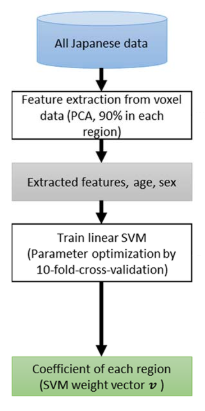
\includegraphics[
    %                         height=6cm
    %                     ]{data/bp_generalization_before.png}
    %                 };
    %             }
    %             \onslide<7->{
    %                 \node[inner sep=0pt, draw=black,anchor=west] at (2, -3) {
    %                     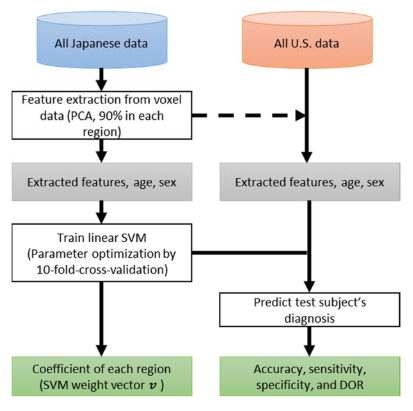
\includegraphics[
    %                         height=6cm
    %                     ]{data/bp_generalization.png}
    %                 };
    %             }
    %             \onslide<6->{
    %                 \node[red] (insample) at (1, -3.66) {88.1\%};
    %                 \draw[-stealth,red,thick] ($ (insample.east) + (0.63, 0) $) -- (insample);
    %             }
    %             \only<8>{
    %                 \node[red] (outofsample) at (9.06, -5.5) {58.3\%};
    %                 \draw[-stealth,red,thick] ($ (outofsample.west) - (0.63, 0) $) -- (outofsample);
    %             }

    %         }
    %     \end{tikzpicture}
    % \end{frame}


    % \begin{frame}{Challenges: Predictive targets}
    %     \begin{tikzpicture}
    %         \node[] at (0, 0) {};
    %         \node[] at (10, -7) {};



    %         \only<1-4>{
    %             \node[] at (5, -5.15) {\scriptsize{Marquand et al., 2016}};
    %             \node[font=\tiny, align=center, anchor=south] at (5, -7.65) {
    %                 Marquand, A. F., Rezek, I., Buitelaar, J., \& Beckmann, C. F. (2016). Understanding heterogeneity in clinical cohorts using normative\\models: beyond case-control studies. Biological psychiatry, 80(7), 552-561
    %             };
    %             \node[inner sep=0pt, anchor=north west] (a) at (1, 0) {
    %                 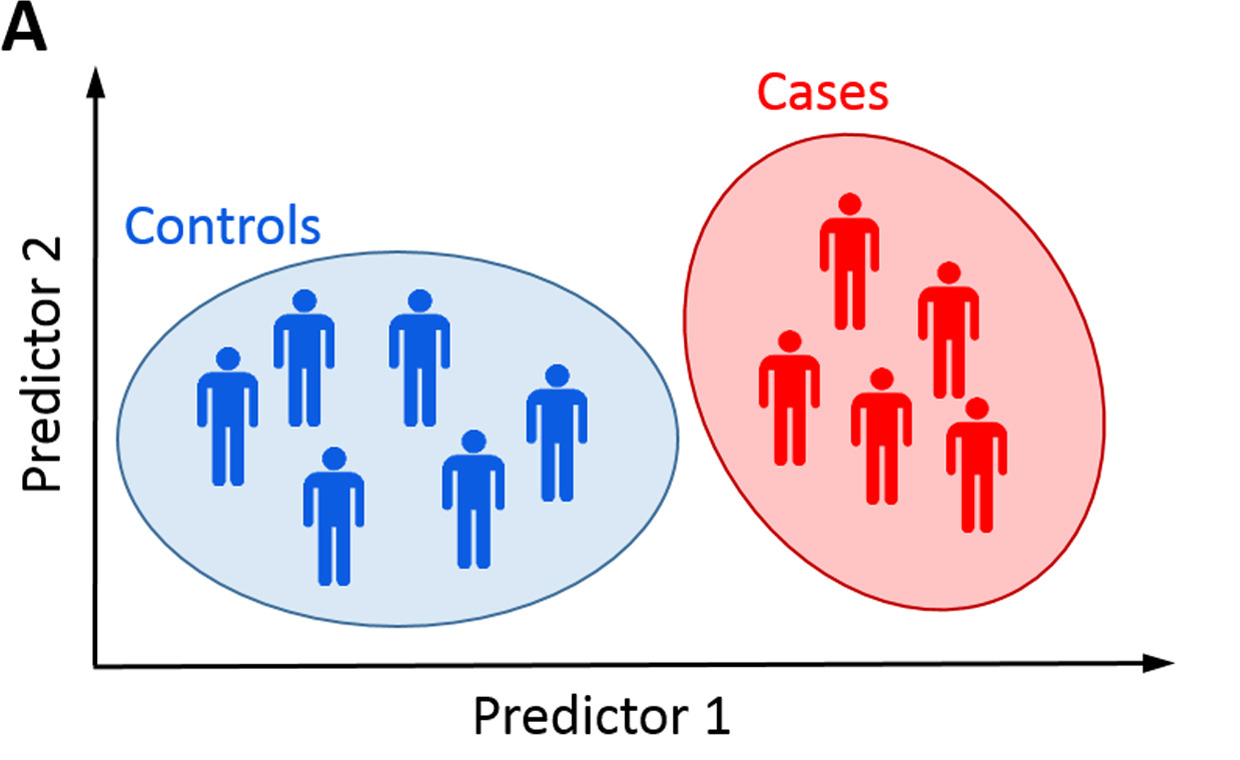
\includegraphics[width=4cm]{data/marquand_a.png}
    %             };
    %             \only<1>{
    %                 \draw[] (a.north west) -- (a.north east) -- (a.south east) -- (a.south west) -- cycle;
    %             }
    %         }
    %         \onslide<2-4>{
    %             \node[inner sep=0pt, anchor=west] (b) at (a.east) {
    %                 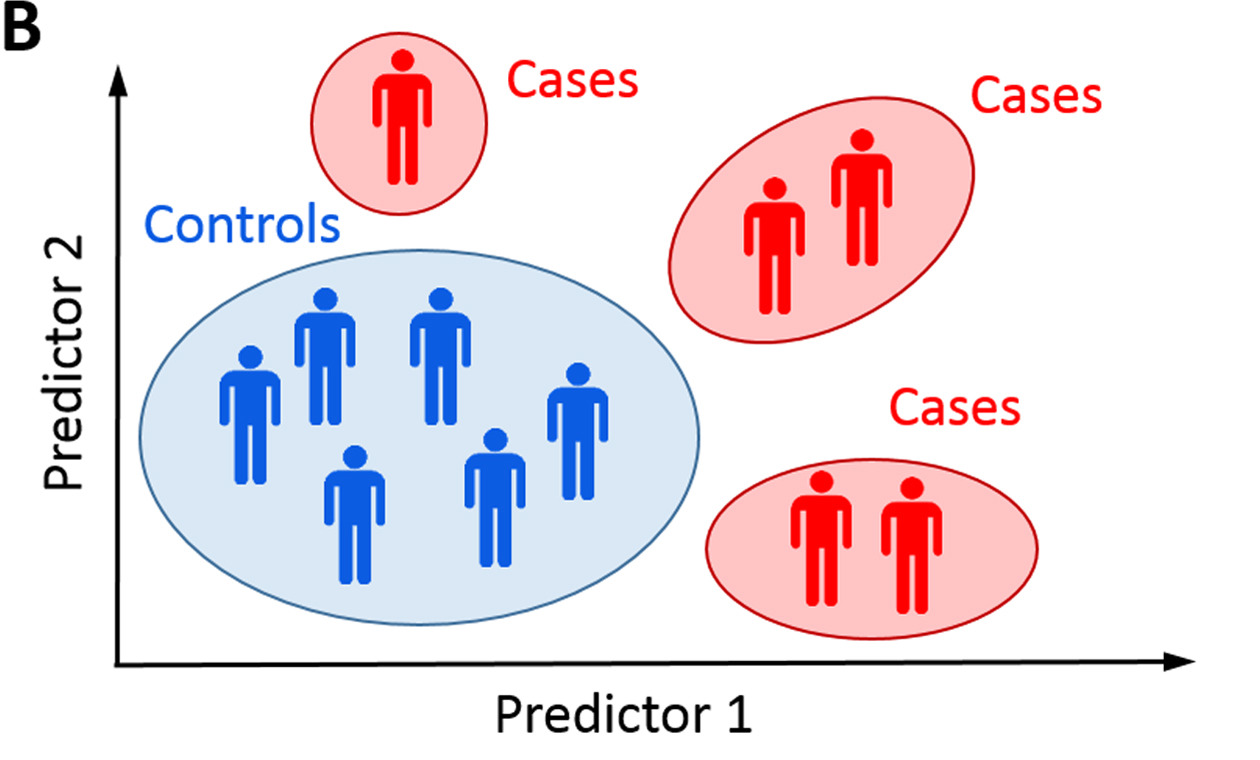
\includegraphics[width=4cm]{data/marquand_b.png}
    %             };
    %             \only<2>{
    %                 \draw[] (a.north west) -- (b.north east) -- (b.south east) -- (a.south west) -- cycle;
    %             };
    %         }
    %         \onslide<3-4>{
    %             \node[inner sep=0pt, anchor=north] (c) at (a.south) {
    %                 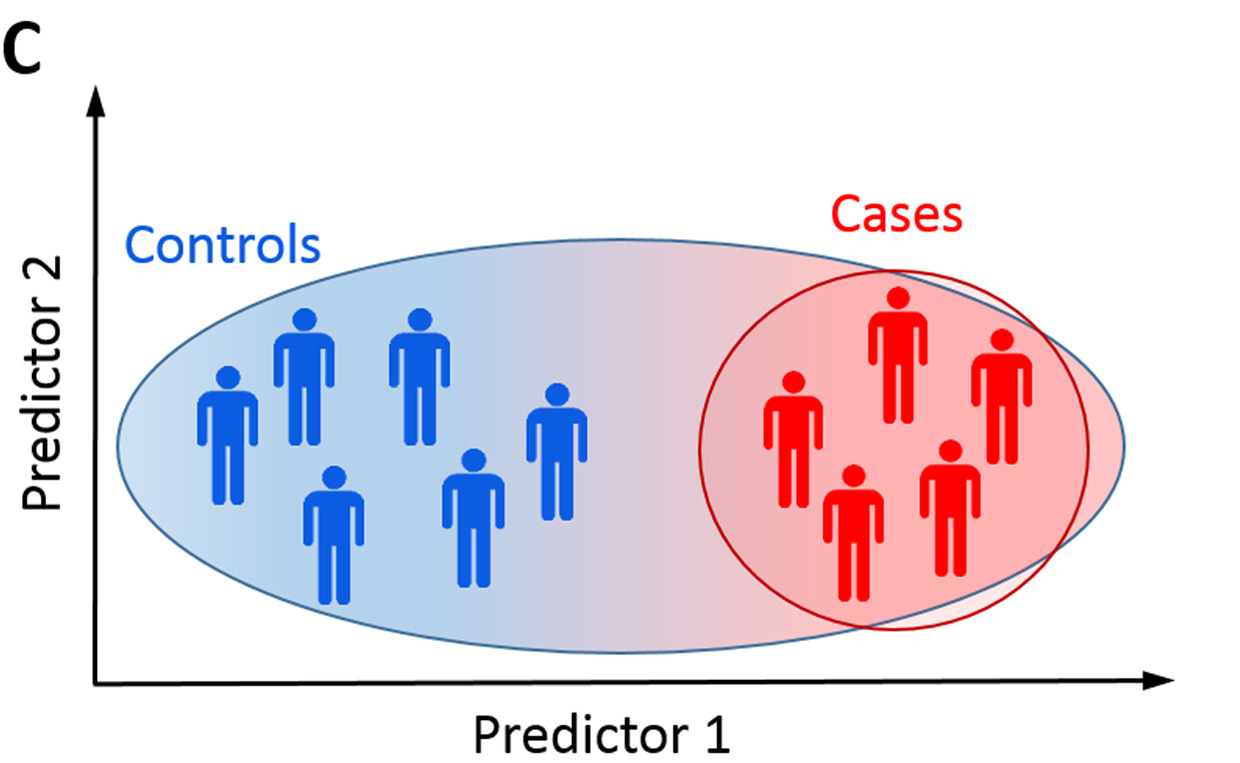
\includegraphics[width=4cm]{data/marquand_c.png}
    %             };
    %             \only<3>{
    %                 \draw[] (a.north west) -- (b.north east) -- (b.south east) -- (b.south west) -- (c.south east) -- (c.south west) -- cycle;
    %             };
    %         }
    %         \only<4>{
    %             \node[inner sep=0pt, anchor=north] (d) at (b.south) {
    %                 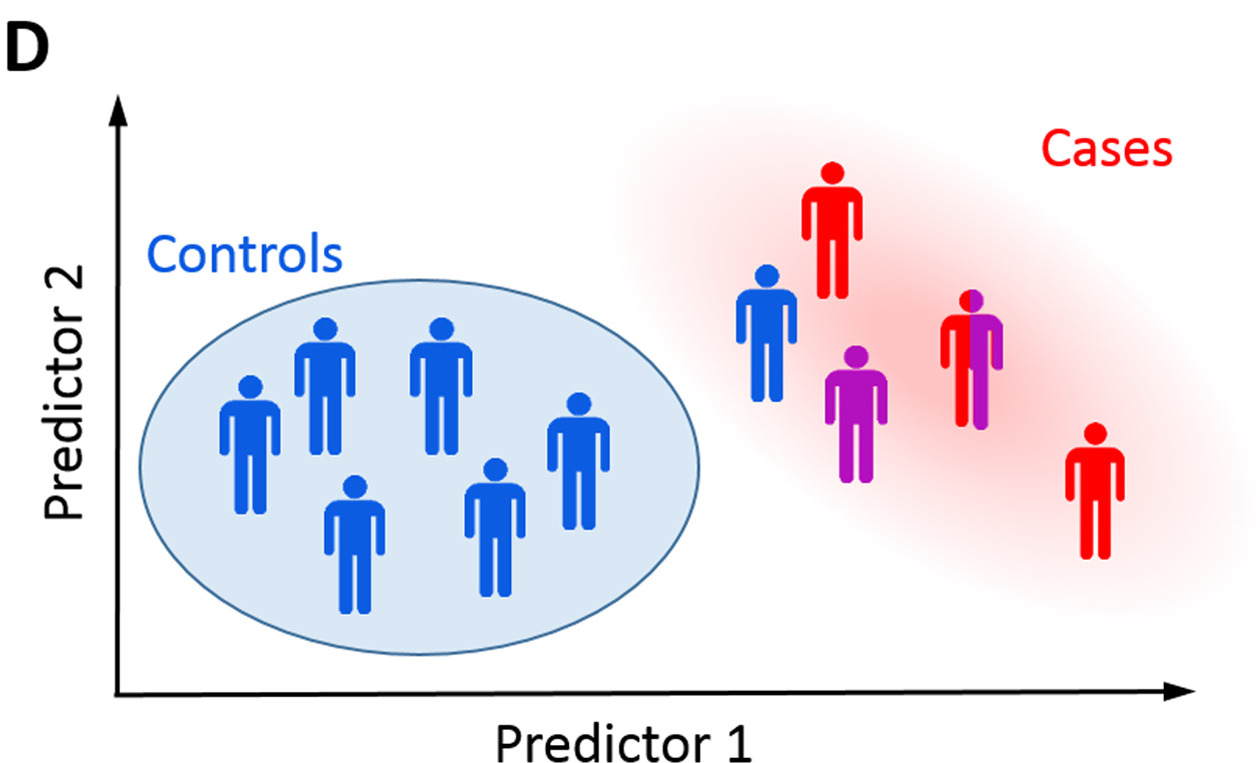
\includegraphics[width=4cm]{data/marquand_d.png}
    %             };
    %             \draw[] (a.north west) -- (b.north east) -- (d.south east) -- (c.south west) -- cycle;

    %         }
    %         \only<5>{
    %             \node[] at (5, -3.5) {
    %                 Diagnostic labels vs prognosis, treatment, differential
    %             };
    %         }
    %     \end{tikzpicture}
    % \end{frame}

    % \newsavebox{\nezer}
    % \sbox{\nezer}{%
    %     \begin{tikzpicture}
    %         \begin{axis}[
    %             height=6cm,
    %             width=8cm,
    %             xtick={1,2,3,4,5,6,7,8,9},
    %             xticklabels={H7,H8,H9,H2,H3,H4,H6,H1,H5},
    %             ymin=0,
    %             ymax=1,
    %             xtick pos=left,
    %             ytick pos=bottom,
    %             x tick style={draw=none},
    %             xlabel=Hypothesis,
    %             ylabel style={align=center},
    %             ylabel={Fraction of teams reporting\\a significant result}
    %         ]
    %             \addplot[
    %                 only marks,
    %                 mark=*,
    %                 mark options={
    %                     draw=black,
    %                     fill=color1,
    %                     opacity=0.8
    %                 },
    %                 mark size=2.5pt,
    %                 error bars/.cd,
    %                 y dir=both,
    %                 y explicit,
    %             ] table [
    %                 x=id,
    %                 y=fv,
    %                 y error plus expr=\thisrow{fv_95u}-\thisrow{fv},
    %                 y error minus expr=\thisrow{fv}-\thisrow{fv_95l},
    %                 col sep=comma
    %             ] {data/botvinik_nezer.csv};
    %         \end{axis}
    %     \end{tikzpicture}
    % }

    % \begin{frame}{Challenges: Preprocessing and degrees of freedom}
    %     \begin{tikzpicture}
    %         \node[] at (0, 0) {};
    %         \node[] at (10, -7) {};

    %         \only<1>{
    %             \node[inner sep=0pt, draw=black, label=below:{\scriptsize{Nørgaard et al., 2020}}] at (5, -3.5) {
    %                 \includegraphics[width=9cm]{data/nørgaard.jpeg}
    %             };

    %             \node[font=\tiny, align=center, anchor=south] at (5, -7.65) {
    %                 Nørgaard, M., Ganz, M., Svarer, C., Frokjaer, V. G., Greve, D. N., Strother, S. C., \& Knudsen, G. M. (2020). Different\\preprocessing strategies lead to different conclusions: a [11C] DASB-PET reproducibility study. Journal of Cerebral\\Blood Flow \& Metabolism, 40(9), 1902-1911
    %             };
    %         }

    %         \onslide<2->{
    %             \node[label=below:{\scriptsize{Adapted from Botvinik-Nezer et al., 2020}}] at (5, -2.7) {
    %                 \usebox{\nezer}
    %             };

    %             \node[font=\tiny, align=center, anchor=south] at (5, -7.65) {
    %                 Botvinik-Nezer, R., Holzmeister, F., Camerer, C. F., Dreber, A., Huber, J., Johannesson, M., ... \& Rieck, J. R. (2020). Variability\\in the analysis of a single neuroimaging dataset by many teams. Nature, 582(7810), 84-88
    %             };
    %         }
    %         \onslide<3>{
    %             \node[minimum width=9cm, minimum height=6cm,fill=black!2,opacity=0.85] at (5, -2.7) {};
    %             \node[fill=none,align=center] at (5, -3) {\textit{"On average across the 9 hypotheses, 20\% of teams reported}\\ \textit{a result that differed from the majority of teams. Given that}\\ \textit{the maximum possible variation is 50\%, the observed fraction}\\ \textit{of 20\% divergent results thus \textbf{falls midway between complete}}\\ \textit{\textbf{consistency across teams and completely random results},}\\ \textit{demonstrating that analytical choices have a major effect on}\\ \textit{reported results."}};

    %         }
    %     \end{tikzpicture}
    % \end{frame}

    % \begin{frame}{Challenges: Interpretability}
    % \end{frame}

    % \begin{frame}
    %     \begin{tikzpicture}
    %         %https://doi.org/10.1007/s40708-015-0019-x
    %         \node[inner sep=0pt, draw=black] at (0, 0) {
    %             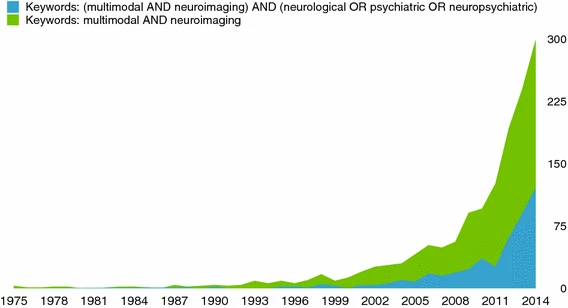
\includegraphics[width=4cm]{data/multimodal_progress.png}
    %         };
    %     \end{tikzpicture}
    % \end{frame}
    % \begin{frame}{The role of prediction}
    %     \centering
    %     \begin{tikzpicture}
    %         %https://doi.org/10.1038/s41380-022-01635-2
    %         \node[inner sep=0pt, draw=black] at (0, 0) {
    %             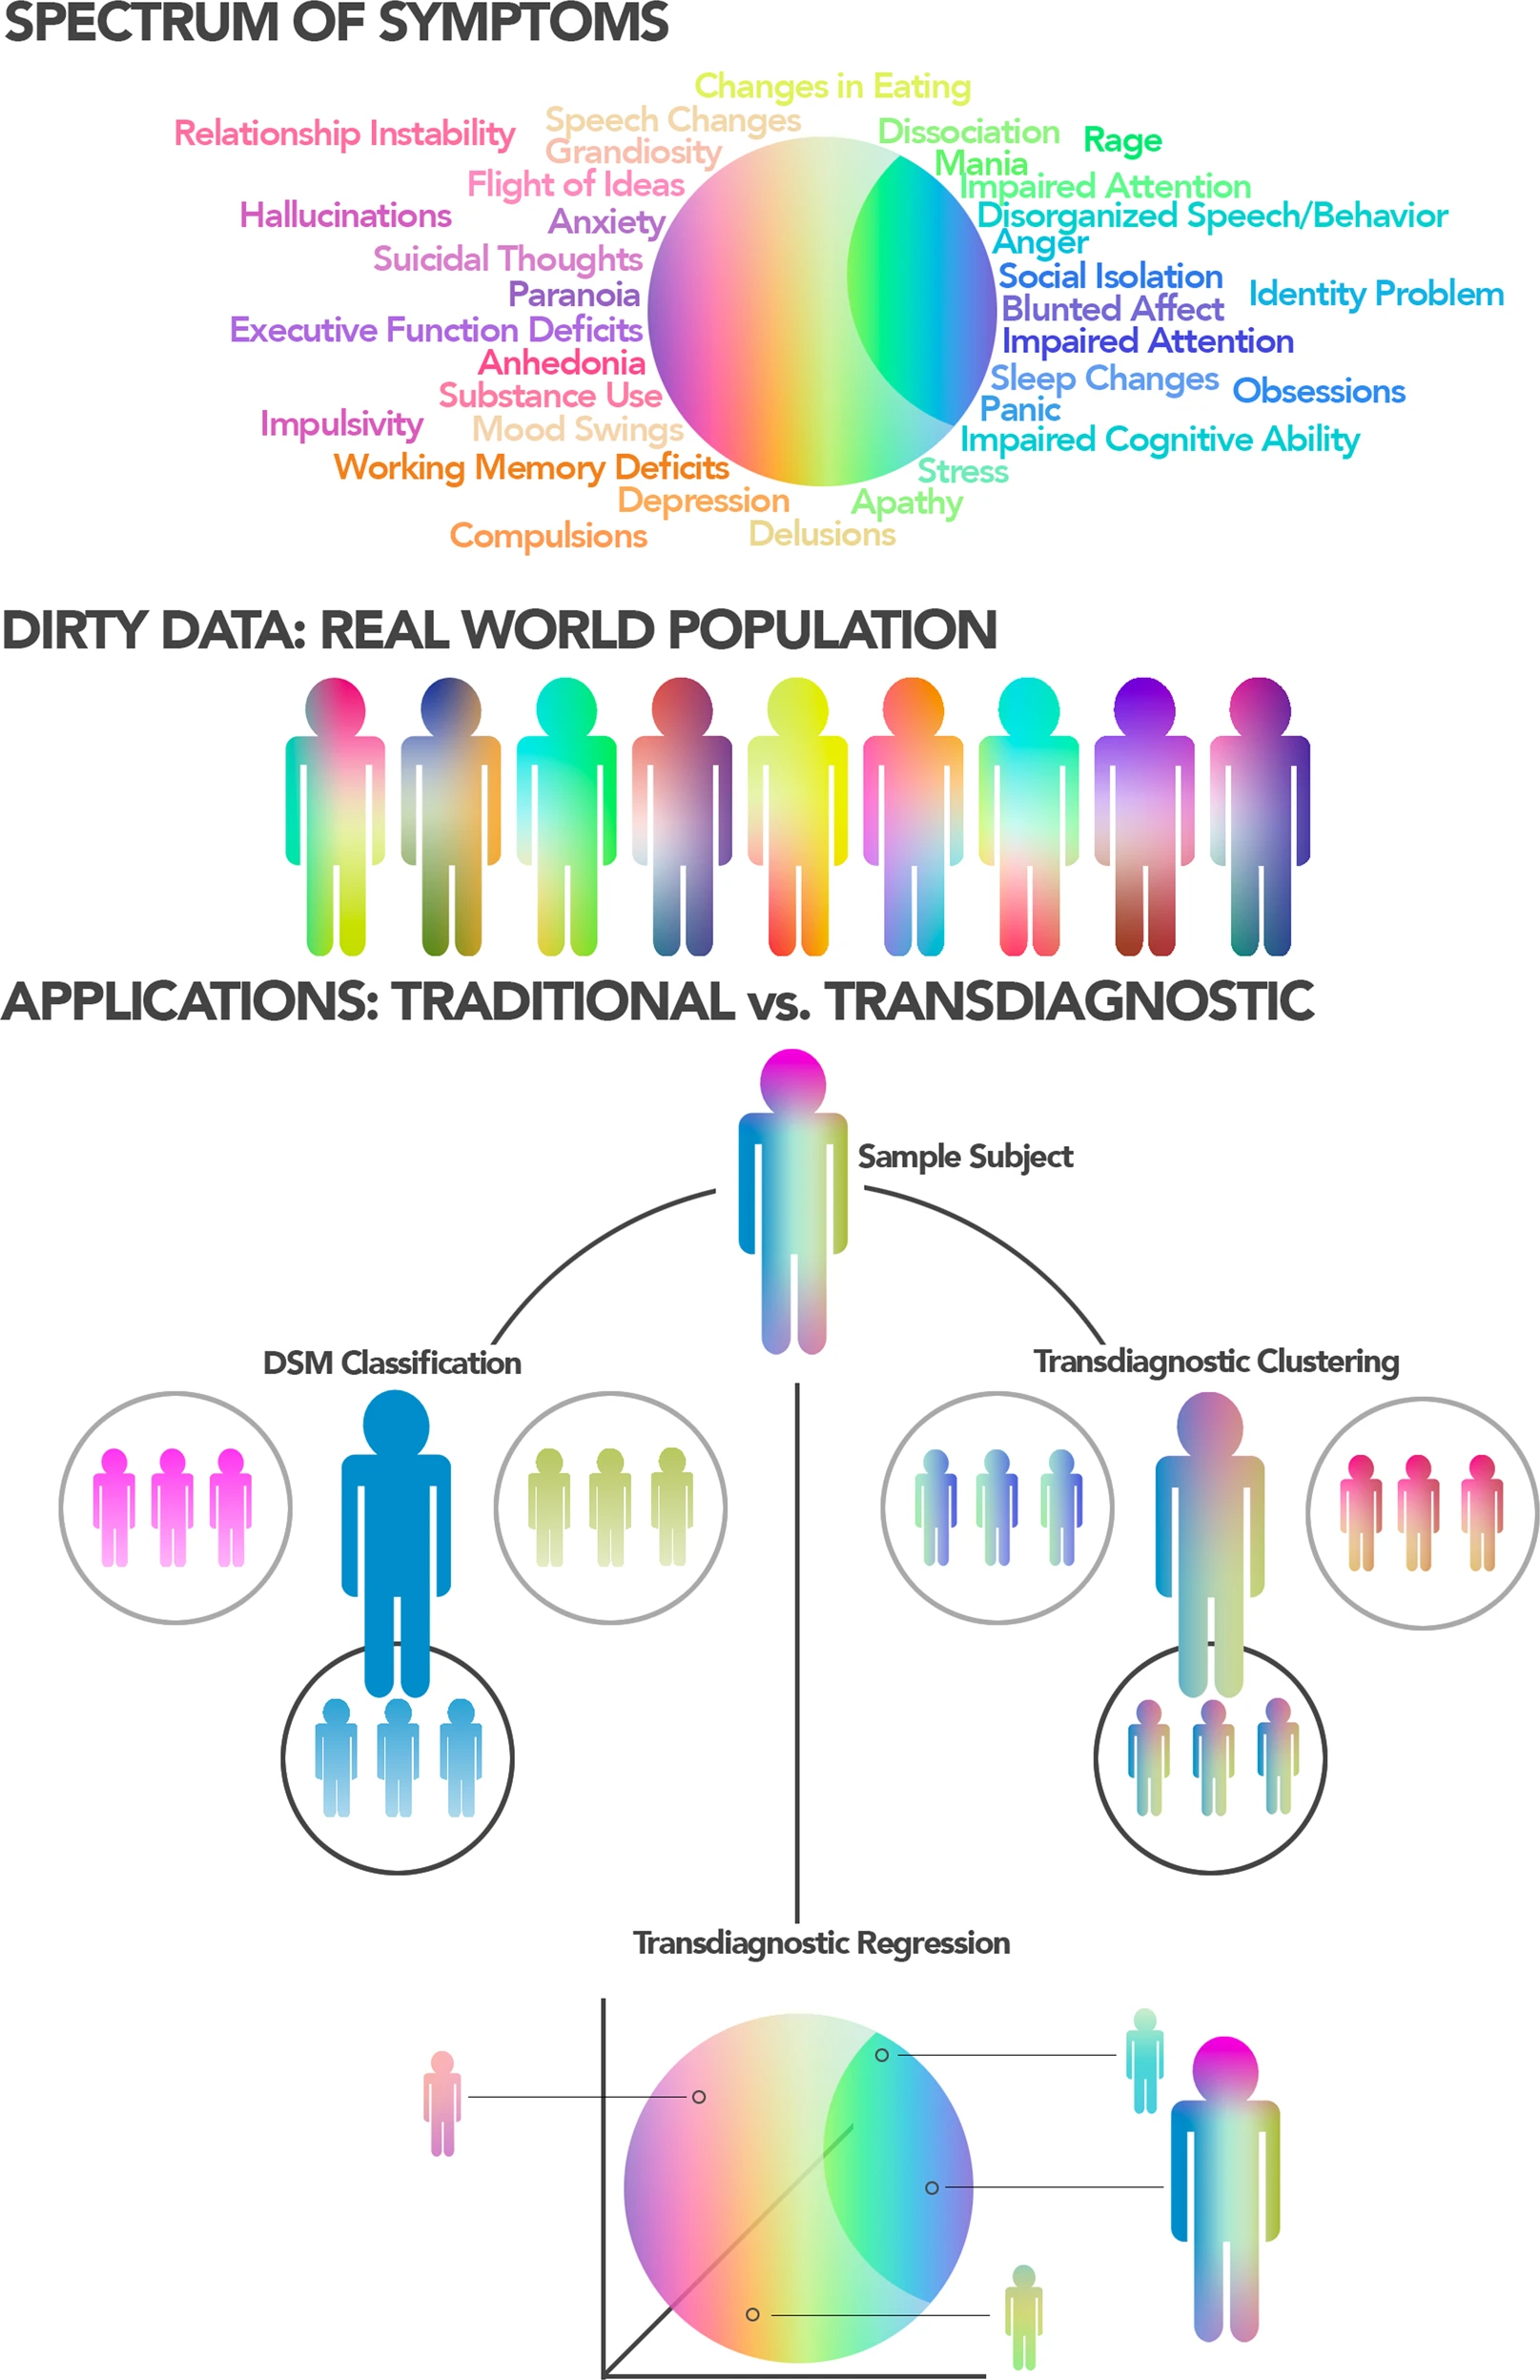
\includegraphics[width=4cm]{data/transdiagnostic.png}
    %         };
    %     \end{tikzpicture}
    % \end{frame}


    % \begin{frame}{Prediction versus interpretability}
    %     \centering
    %     \begin{tikzpicture}
    %         %https://doi.org/10.1038/s41380-022-01635-2
    %         \node[inner sep=0pt, draw=black] at (0, 0) {
    %             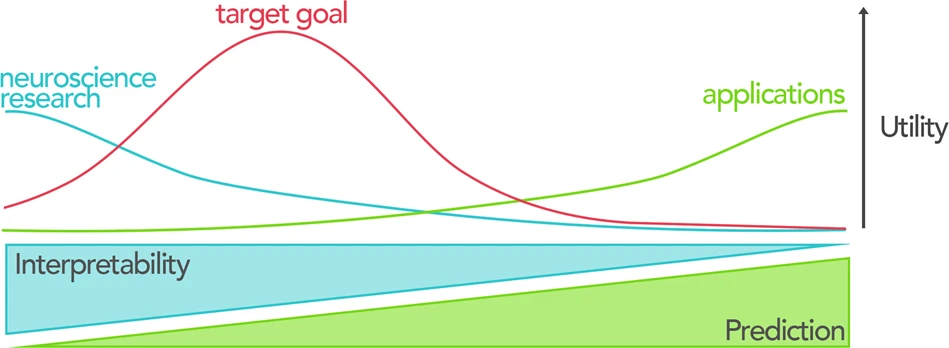
\includegraphics[width=8cm]{data/prediction_vs_interpretability.png}
    %         };
    %     \end{tikzpicture}
    % \end{frame}
\end{document}
